% --- Template for thesis / report with tktltiki2 class ---
% 
% last updated 2013/02/15 for tkltiki2 v1.02

\documentclass[english, grading]{tktltiki2}

% tktltiki2 automatically loads babel, so you can simply
% give the language parameter (e.g. finnish, swedish, english, british) as
% a parameter for the class: \documentclass[finnish]{tktltiki2}.
% The information on title and abstract is generated automatically depending on
% the language, see below if you need to change any of these manually.
% 
% Class options:
% - grading                 -- Print labels for grading information on the front page.
% - disablelastpagecounter  -- Disables the automatic generation of page number information
%                              in the abstract. See also \numberofpagesinformation{} command below.
%
% The class also respects the following options of article class:
%   10pt, 11pt, 12pt, final, draft, oneside, twoside,
%   openright, openany, onecolumn, twocolumn, leqno, fleqn
%
% The default font size is 11pt. The paper size used is A4, other sizes are not supported.
%
% rubber: module pdftex

% --- General packages ---

\PassOptionsToPackage{hyphens}{url}
\usepackage[hyphens]{url}
\usepackage[utf8]{inputenc}
\usepackage[T1]{fontenc}
\usepackage{lmodern}
\usepackage{microtype}
\usepackage{bbm} % indicator
\usepackage{amsfonts,amsmath,amssymb,amsthm,booktabs,color,enumitem,graphicx}
\usepackage[pdftex,hidelinks]{hyperref}
\usepackage{longtable}
\usepackage{listings}
\usepackage{diagbox}
\usepackage{array}


\usepackage{pgfplots}
\pgfplotsset{compat=1.15}
\newlength\figureheight
\newlength\figurewidth

%tikz
\usetikzlibrary{shapes.geometric, arrows}
\tikzstyle{startstop} = [rectangle, rounded corners, minimum width=3cm, minimum height=1cm,text centered, draw=black]
\tikzstyle{io} = [trapezium, trapezium left angle=70, trapezium right angle=110, minimum width=3cm, minimum height=1cm, text centered, draw=black]
\tikzstyle{process} = [rectangle, minimum width=3cm, minimum height=1cm, text centered, draw=black]
\tikzstyle{decision} = [diamond, minimum width=3cm, minimum height=1cm, text centered, draw=black]
\tikzstyle{arrow} = [thick,->,>=stealth]

\usepackage{hhline}

\usepackage{parcolumns}
\usepackage{multicol}
\usepackage{multirow}
\usepackage{subcaption}

\usepackage{qtree}
\usepackage{newfloat}
\DeclareFloatingEnvironment[fileext=lod]{diagram}

\usepackage{dirtytalk}

\usepackage{algorithm}
\usepackage{algpseudocode}
%\usepackage[bottom]{footmisc}

% Automatically set the PDF metadata fields
\makeatletter
\AtBeginDocument{\hypersetup{pdftitle = {\@title}, pdfauthor = {\@author}}}
\makeatother

% --- Language-related settings ---
%
% these should be modified according to your language

% babelbib for non-english bibliography using bibtex
\usepackage[fixlanguage]{babelbib}
\selectbiblanguage{english}

% add bibliography to the table of contents
\usepackage[nottoc]{tocbibind}
% tocbibind renames the bibliography, use the following to change it back
\settocbibname{References}


% -- Handy shortcuts
\newcommand{\etal}{\textit{et al}. }
\newcommand{\ie}{\textit{i}.\textit{e}., }
\newcommand{\eg}{\textit{e}.\textit{g}. }
\newcommand{\cpp}{C\texttt{++}}
\newcommand{\bolditt}[1]{\mathbf{#1}}
\newcommand{\norm}[1]{\left\lVert#1\right\rVert}

\DeclareMathOperator*{\argmax}{argmax}
\DeclareMathOperator*{\argmin}{argmin}

% --- Theorem environment definitions ---
\newtheorem{lau}{Lause}
\newtheorem{lem}[lau]{Lemma}
\newtheorem{kor}[lau]{Korollaari}

\theoremstyle{definition}
\newtheorem{maar}[lau]{Definition}
\newtheorem{ong}{Ongelma}
\newtheorem{alg}[lau]{Algoritmi}
\newtheorem{esim}[lau]{Esimerkki}
\newtheorem{example}{Example}

% algorithmic
\algnewcommand\algorithmicinput{\textbf{Assume:}}
\algnewcommand\Assume{\item[\algorithmicinput]}

\theoremstyle{remark}
\newtheorem*{huom}{Huomautus}

\numberwithin{equation}{section} % equations as (chapter num. , i)

% --- tktltiki2 options ---
%
% The following commands define the information used to generate title and
% abstract pages. The following entries should be always specified:

\title{Automatic Software Plagiarism Detection}
\author{Kristian Wahlroos}
\date{\today}
\level{M.Sc. Thesis}
\abstract{
Plagiarism is an act of copying where one doesn't rightfully credit the original source. The motivations behind plagiarism can vary from gaining economical advantage to even completing academic courses in a desperate way. Plagiarism itself exists in various domains where people want to take credit from something they have worked on. These areas can include e.g. literature, art or software.   

In this study, automatic authorship identification and plagiarism detection from software is analyzed and a model is built on top of findings. The term \textit{automatic} here refers to a system which requires as little as possible human intervention as possible. The goal for the model is to point out possible plagiarism from a collection of documents, which here is specified as a collection of source code files written by various authors. This situation closely related to authorship identification, and thus as a statistical tool, supervised machine learning model is utilized. The latter problem can be stated as \emph{given a document, which author has written this} and \emph{does this document follow the previous style of the author}. 
}

% The following can be used to specify keywords and classification of the paper:

\keywords{plagiarism; authorship identification; }

% classification according to ACM Computing Classification System (http://www.acm.org/about/class/)
% This is probably mostly relevant for computer scientists
% uncomment the following; contents of \classification will be printed under the abstract with a title
% "ACM Computing Classification System (CCS):"
% \classification{}

% If the automatic page number counting is not working as desired in your case,
% uncomment the following to manually set the number of pages displayed in the abstract page:
%
% \numberofpagesinformation{16 sivua + 10 sivua liitteissä}
%
% If you are not a computer scientist, you will want to uncomment the following by hand and specify
% your department, faculty and subject by hand:
%
% \faculty{Matemaattis-luonnontieteellinen}
% \department{Tietojenkäsittelytieteen laitos}
% \subject{Tietojenkäsittelytiede}
%
% If you are not from the University of Helsinki, then you will most likely want to set these also:
%
% \university{Helsingin Yliopisto}
% \universitylong{HELSINGIN YLIOPISTO --- HELSINGFORS UNIVERSITET --- UNIVERSITY OF HELSINKI} % displayed on the top of the abstract page
% \city{Helsinki}
%



% 10-15 pages abstract

\begin{document}

\lstdefinestyle{mystyle}{
    tabsize=2,
    breakatwhitespace=false,         
    breaklines=true,                 
    keepspaces=true,
    %numbers=left,
    showspaces=false,                
    showstringspaces=false,
    showtabs=false,
    numberstyle=\small,
    numbersep=8pt,
    columns=flexible,
    %framexleftmargin=15pt,
    xleftmargin=\parindent,
    basicstyle=\ttfamily\small,
    keywordstyle=\color{red}
}
 
\lstset{style=mystyle}


% --- Front matter ---

\frontmatter      % roman page numbering for front matter

\maketitle        % title page
\makeabstract     % abstract page

\tableofcontents  % table of contents

% --- Main matter ---

\mainmatter       % clear page, start arabic page numbering

\section{Introduction}

%What means term plagiarism?
%What is plagiarism?
%Why studied here --> 

Massive Online Courses (MOOCs) are a popular way to complete undergraduate courses offered by various institutes and universities. For example a course \emph{Circuits and Electronics} led by Massachusetts Institute of Technology and Harvard University, gathered around 155\,000 registered students from all over the world to a website called \emph{edX}\footnote{\url{https://www.edx.org/}} in 2012 \cite{SLWCRFM2013}. The structure of \emph{Circuits and Electronics} consisted of two parts which are now common in majority of MOOCs: theory part and graded tasks which are offered weekly during the timespan of a course. 

The course \emph{Ohjelmoinnin MOOC} is an online programming course offered by University of Helsinki. It has a two-parted structure, introduction and advanced course in Java programming language, where both are mandatory undergraduate-level courses split into seven weeks of total workload. During these weeks students follow the offered course material independently and submit their solutions to various programming tasks that are automatically tested and scored. If the participant is not a registered student in University of Helsinki, he/she can apply for a study right after completing the course and taking an exam, otherwise the student gains total of ten credits to his/her degree. 

As the nature of \emph{Ohjelmoinnin MOOC} is heavily score-based and students are free to choose their working hours without any major mandatory attendance, it can create a motivation to cheat among  students. Also the fact that there are over hundred students registered and many submissions sent by each student, makes it practically impossible for course staff to detect possible cheating. 

The word \emph{cheating} here refers to an act of plagiarism and one of the ways to define the verb \emph{plagiarize} is as \say{to steal and pass off (the ideas or words of another) as one's own}\footnote{\url{https://www.merriam-webster.com} Accessed 10th April 2018}, and the person conducting this act is called \emph{a plagiarist}. Source-code plagiarism on other hand, refers to the act of plagiarism that happens between software that is built from various source code documents. This kind of plagiarism can be also defined as \emph{source-code reuse}, which includes the following four facets \cite{TDSCP2008}: copying others work without alterations, copying and changing some parts of the code to fool a human inspector, converting a solution from one language to another and using code-generators to automatically create a solution. 


Source-code plagiarism in academia is considered as a serious offence and there often exists a zero tolerance for it \cite{TDSCP2008}. This is usually stressed at the start of courses and can lead to serious consequences ranging from rejecting the students current course registration to even suspension. Dick \etal points out that in some cases over 80\% of the students were found guilty of cheating if they were given a good enough opportunity for it \cite{Dick:2002:ASC:782941.783000}. Usual forms of cheating methods were found to be related to plagiarism: copying solutions from the web, sharing solutions with friends and excessive collaboration between students. 

The opinions about cheating motives varies between students and academics \cite{TDSCP2008}. Academics reported that cheating is due to three major factors: external pressure, the ease of sharing solutions and cultural differences. Students on the other hand, gave two major reasons: time pressure and heavy workloads. Now given also the MOOCs time sensitive weekly assignments, the automatic scoring system, and freedom to complete the course wherever students want, can give a motivation to cheat.

In this study we approach the problem of source code plagiarism detection with data mining and machine learning. By data mining we mean an approach that is able to use computers to find interesting patterns from the data, and by machine learning a statistical process which is able to make predictions using computers. For our proposed detection model, we first build two classifiers: identifying suspicious authors based on the similarity scores obtained from documents and authorship identification that is able to predict the most likely author of a document. Suspicious authors are grouped together to reveal clusters of possible plagiarists, whereas authorship identification is used to detect if a writing style of an author matches to his/her previous work. Using results from both of these classifiers, we propose our approach where the intersection between suspicious authors and candidate authors given a document, is able to reveal cases of possible plagiarism from a set of source codes.

Following three research questions are asked and answered in this study, which are all tied closely to the question \emph{How plagiarism can be automatically detected?}

\begin{itemize}
    \item[Q1:] \emph{What kind of approaches exist to detect source code plagiarism?}
    \item[Q2:] \emph{What are the possible benefits of using code structure for plagiarism detection?}
    \item[Q3:] \emph{How one can reduce the amount of false accusations?}
\end{itemize}

\noindent
To answer these questions, we first conduct a literature review in which we establish a categorization for various techniques and base our approach to findings. Then, we will show how the code structure can be used within detection and what are the theoretical benefits of doing so. Finally, we will evaluate our approach which combines both structural and high-level information about source code, to see if the rate of false positives decreases when using similarity detection with authorship identification contrast to using only either one.
%needs rewriting

Rest of this study is structured as follows: in Chapter 2 more detailed overview of source code plagiarism is given with a theory of classifiers, Chapter 3 presents the results of systematic literature review where we focus on data and methods applied in research, in Chapter 4 our method of using the result of two classifiers and the used real-life data sets are presented, Chapter 5 presents the results by comparing our method to two popular baselines answering previous research questions. Chapter 6 discusses the results, shortcomings with our proposal and possible problems when automatic system is used to accuse students from plagiarism. 

\section{Background}

In this chapter we define the problem of plagiarism detection more formally, describe possible plagiarism strategies and give an overview of the similarity detection and authorship identification. We will approach these latter two problems by first defining them, then showing how they tie closely to the domain of information retrieval, and finally giving two real-life models. The first model is a probabilistic model able to predict the author based on the authors previous work, and the second model is a clustering algorithm which can group similar documents together. We start first by defining the problem of plagiarism detection.    

\newtheorem*{sc-plg}{Plagiarism detection}
\begin{sc-plg}
Given a set of documents $D = \{d_1, d_2, ..., d_n\}$ called as the corpus and a set of authors $A = \{a_1, a_2, ..., a_k\}$ who are writers of these documents, define a function $f$ that is able to classify which documents are plagiarized, and who are possible plagiarists from the set of authors $A$.
\end{sc-plg}

Above formalization gives an overview of the problem that is studied in this thesis, and some aspects about the problem have been simplified for this study. For example we don't try to reveal the \emph{direction} of plagiarism, we ignore any possible data gathered from the creation process and we only consider authors inside a predefined set. This means that we try only to detect if possible plagiarism can be observed from the textual representation, which can be interpreted as the collection of student submissions.  

To get a better understanding of the details that are relevant to source-code plagiarism, instead of \eg detecting plagiarism from essays, we define some important themes and terms next. Starting from the definition of source code plagiarism, we show some common strategies of plagiarists and briefly introduce the underlying structure of a source code and existing tools to detect plagiarism.

\subsection{Source-code plagiarism}

Source-code plagiarism refers to a plagiarism that happens between source code files. This 
scenario is common in academic programming courses and in software industry, where detection can be impossible due to time constraints. In academia, the underlying motives behind source code plagiarism include things like \cite{DPPA2008}; ambiguity about what is considered as excessive collaboration between students, using other students work to gain grades and minimizing the work needed to complete the course. Also, some students have problems to define what they consider as source-code plagiarism, and thus three common guidelines can be given \cite{Pieterse2014DecodingCP}:

\begin{enumerate}
    \item[1)] Refactoring other students work, and submitting it as your own, is plagiarism
    \item[2)] If exercise templates are used, possible similarities between documents and templates are not plagiarism
    \item[3)] Submitting a direct copy of other students work is plagiarism
\end{enumerate}

\noindent
%Because of possible confusion about what is considered as plagiarism and the serious nature of plagiarism accusations in academia, it's preferable still to use some kind of human expert to judge to call out if a student has actually plagiarized someone \cite{Pieterse2014DecodingCP}. This allows the detection process to reveal candidates, which prunes heavily the amount of manual work needed.
Detecting 2. and 3. are straightforward; code templates can be filtered out from documents so that they contain only students own work and detecting direct copy can be easily found by using string matching techniques. However, the problem arises when students tries to hide the plagiarism by mutating the copied document.

\paragraph{Plagiarism strategies}\mbox{}\\
Some common source code transformation techniques, often called as \emph{obfuscation strategies}, are targeted mainly towards two types of changes \cite{DPPA2008}: lexical and structural. Lexical changes doesn't require a deeper understanding of the logic and are doable with any \emph{integrated development environment} (IDE). Structural changes requires some understanding of the program logic, and includes modifications which change the layout of the source code but keeps the logic same. For example considering clause with an operand \texttt{if(a == true)}, this can be written equally as \texttt{if(a == !false)}.

\begin{table}[ht]
\centering
\caption{Common transformation targets.}
\label{tbl-plag-strat}
\begin{tabular}{|l|l|} \hline
 \textbf{Lexical} & \textbf{Structural} \\ \hhline{|=|=|}
 Comments                    & Loops                          \\
 Formatting                  & Clauses                        \\
 Naming                      & Statement order                \\
                             & Operand order               \\ \hline
\end{tabular}
\end{table}

Table \ref{tbl-plag-strat} shows some of the most common transformation targets in source codes. Given a source code from another student, plagiarist can apply above transformations and complicate the task for a human to spot plagiarism, or even confuse naïve methods. The motivation behind using these transformations is simple, plagiarists want to hide traces and thus, the detection method must be resilient against these strategies.


Plagiarism transformations defined in table \ref{tbl-plag-strat} closely relate to an earlier study which characterized six levels of transformations \cite{Faidhi:1987:EAD:27319.27321}.

\begin{table}[ht]
\centering
\caption{Transformation levels.}
\label{tbl-plag-transf}
\scalebox{0.85}{
    \begin{tabular}{|c||c|p{5cm}|} \hline
     \textbf{Level of change} & \textbf{Target}  & \textbf{Example action}\\ \hhline{|=|=|=|}
     1 & Comments and indentation & Add extra spaces and newlines\\ \hline
     2 & Identifiers & Rename all variables\\ \hline
     3 & Declarations & Reorder functions\\ \hline
     4 & Modules & Merge functions\\ \hline
     5 & Statements & Use \texttt{for} instead of \texttt{while}\\ \hline
     6 & Logic & Change whole expressions\\ \hline
    
    \end{tabular}
    }
\end{table}

\noindent
Applying all of these transformations one after another, makes the detection of plagiarism very difficult, as the plagiarized document diverges too much from the original document and hides most of the traces that could be used for detection. However, as the textual information changes, plagiarists still try to maintain the same logic between original and copied documents. This implies that there still exists some kind of similarity, but now the similarity can't be found directly from the textual representation of a source code. Information about the logical structure is thus crucial and accessible when source code is parsed to a tree format.

\paragraph{Code structure}\mbox{}\\
Source code is a structured text, made of keywords and user-defined variables. To write a running program, one must know the rules \ie the \emph{grammar} of a language, which is usually represented as the order in which various keywords and variables must follow each others. A compiler is the core of a programming language and is able to transform a source code into a machine code. When rules must be interpreted by the compiler, it uses a \emph{parse tree} that is generated from the source code \cite{johnson1975yacc}. This parse tree captures the syntax and semantics of a source and the abstracted version of it, is called \emph{abstract syntax tree}. Consider for example storing an integer value to a variable, the source code and its syntax tree is visible from the following diagram.

\begin{diagram}[ht]
\centering
\scalebox{1}{
\Tree[.VariableDeclaration [.Identifier "a" ] [.Literal "5" ] ]
}
\caption{Example syntax tree for \texttt{var a = 5;}}
\label{diag-parse}
\end{diagram}

\noindent
Pruning the leaves of diagram \ref{diag-parse} leads to a more general expression that captures the logic of the source code, becoming resistant against most of the transformations given in table \ref{tbl-plag-transf}. This gives ability to detect similar \emph{structure} rather than similar \emph{tokens}, which are more vulnerable to simple transformations.

\paragraph{Tools}\mbox{}\\
Because plagiarism is kept as a serious offence in academia, a lot of various detection software has been made for it. Novak lists seven of the most well-known tools in a review and explains some common properties \cite{RSCAD2016}: \emph{MOSS, JPlag, SPLaT, SIM, Marble, Plaggie} and \emph{Sherlock}. These tools can be classified into five different categories based on methods used: text, token, graph, tree and hybrid. Among these tools, the most common way to detect plagiarism is a five step approach: pre-process documents, tokenize documents, exclude templates, calculate similarities and finding suspects using these similarity scores.

\newpage

\subsection{Similarity detection} \label{chap-sd}

Similarity detection, or code clone detection, focuses directly on finding similar functionality between arbitrary pair of source codes $\{d_i, d_j\}$. We define it formally as following

\newtheorem*{smd1}{Similarity detection}

\begin{smd1}
Given a set of source code documents $D = \{d_1,...,d_n\}$ called corpus, define normalized similarity function $sim: d_i, d_j \rightarrow [0, 1]$ where $1 \leq i, j \leq n$, such that $sim(d_i, d_j) = sim(d_j, d_i)$ and $sim(d_i, d_i) = 1$, with a optional threshold $\theta \in [0, 1]$ that defines the limit where two source codes are considered as too similar. With this definition, any pair of source code file $(d_i, d_j) \in D \times D$ can also be presented as a triplet $(d_i, d_j, s)$, where $s$ is the similarity value between documents. 
\end{smd1}

\noindent
Above definition is flexible enough to support multiple solutions for the same task, the only restriction being that one must define a function that is able to return a score that either captures the textual or functional similarity. Defined method should be as resilient as possible against transformations given in table \ref{tbl-plag-strat} and table \ref{tbl-plag-transf}, so that two logically similar programs will get a high score even if their textual information differs. Scoring here refers to the value given by similarity function, which can be thought as a distance between documents.

The approach one takes, is ultimately based on how source code document is seen as a data \cite{Roy:2009:CEC:1530898.1531101}: document consisting of plain text, series of tokens, syntax tree, series of metrics or as a graph. The textual approach is based on detecting fragments of copy and paste, and requires no pre-processing if one uses naïve methods like string matching. Another way of approaching is by selecting a specific analysis method: attribute-counting-metrics, which are high-level metrics or by structure-metrics which are able to capture more low level representation of the source code \cite{Verco:1996:SDS:369585.369598}. Despite the approach, some kind of pre-processing and normalization is practically always used to prevent the method to be confused with common obfuscation strategies. 

The core process to detect similarity can be visualized as in figure \ref{fig-sd-flow}, which follows the general structure seen in many state of the art systems \cite{Roy:2009:CEC:1530898.1531101}.

\begin{figure}[!ht]
\centering
\vspace{0.5cm}
\scalebox{0.75}{
   \begin{tikzpicture}[node distance=2cm, baseline]

    \node (start) [io] {Corpus};
    \node (pro1) [process, right of=start, xshift=4.1cm] {Pre-process};
    \node (pro2) [process, right of=pro1, xshift=5cm] {Transform};
    \node (pro3) [process, below of=pro2] {Clone detection};
    \node (end) [io, below of=start] {Suspects};
    
    \draw [arrow] (start) --  node[anchor=south] {Raw source code} (pro1);
    \draw [arrow] (pro1) -- node[anchor=south] {Partition} (pro2);
    \draw [arrow] (pro2) -- node[anchor=east] {Intermediate representation} (pro3);
    \draw [arrow] (pro3) -- node[anchor=north] {Pairwise similarity} (end);
    
    \end{tikzpicture}
}
\caption{Similarity detection process}
\label{fig-sd-flow}
\end{figure}

\noindent
In figure \ref{fig-sd-flow} after the corpus has been set, pre-process stage takes as an input the unmodified source codes to perform two key tasks: to remove unnecessary segments and to determine the level of comparison granularity. The granularity one chooses can range from function-level to document-level, depending how accurately the results should pinpoint code reuse. After the source code has been partitioned, it is transformed into intermediate representation which consists of two parts: extraction that transforms the data to be used for clone detection algorithm \eg by parsing, tokenizing or building a control flow; and normalization. In latter one can apply techniques which reduce the noise between source codes: comments and whitespace removal, uniforming user-defined identifiers and/or removing syntactic noise.

The most key issue regarding to similarity detection, are false-positives that can be handled by manual verification after the suspects are gathered \cite{Verco:1996:SDS:369585.369598, Roy:2009:CEC:1530898.1531101}. This is often mandatory as detection algorithms can't completely understand nuances related to actual plagiarism \eg what is considered as being too similar. 


%\begin{minipage}{.45\hsize}
%\begin{lstlisting}[language=Java, caption=Example code 1]{asd1}
%void code()
%{
%
%}
%\end{lstlisting}
%\end{minipage}\hfill
%\begin{minipage}{.45\hsize}
%
%\begin{lstlisting}[language=Java, caption=Example code 2]{asd2}
%void code()
%{
%
%}
%\end{lstlisting}
%\end{minipage}


\subsection{Authorship identification} \label{chap-ai}

Authorship identification deals with the issue of trying to name the author of a document given some previous work of the author. This problem can be seen as a classification task \cite{KRSUL1997233}, thus we can define authorship identification formally as following.

\newtheorem*{aui1}{Authorship identification}
\begin{aui1}
Given a set of documents $D$, a set of authors $A$ and a function $f: D \rightarrow A$ that identifies the writer by assigning every source code document $d \in D$ to one author $a \in A$. Estimate $f$ with $\hat{f}$, a classifier that treats every document as a feature vector $\bolditt{x}$ and every known class as a vector $\bolditt{y}$. The predicted author $\hat{y}$ can be thus expressed with $\hat{f}(\bolditt{x}) = \hat{y}$.
\end{aui1}

\noindent
This classifier should be able to discriminate between writing styles of different authors, which in programming refers to the habits \ie programming style. Habits are restricted by the grammar of the chosen programming language, but commonly refers to everything that is controllable by the author \eg how one names variables or uses spacing. As a problem, it's therefore very opposite to the similarity detection where we want to find maximum equivalency between programs. 

One way to represent programming style is by using software metrics \cite{KRSUL1997233}. Software metrics can be put into roughly three categories: layout being fragile metrics which are easily transformed by the IDE, style which are non-fragile metrics related to layout and lastly structure which can capture experience and ability of the programmer. As source code can be also thought as a text written with a specific language, majority of the methods using a natural language can be applied, thus we can form a five-level categorization for stylistic features called \emph{stylometrics features}  \cite{Stamatatos:2009:SMA:1527090.1527102}. Categorization for stylometric features is visualized in table \ref{tbl-ai-stylomet}, where semantic features are the most difficult to form as they require understanding deeper meaning of the written source code.

\begin{table}[ht]
\centering
\caption{Five-levels of stylometrics features. }
\label{tbl-ai-stylomet}
\begin{tabular}{|c|c|} \hline
\textbf{Category}             & \textbf{Feature examples} \\ \hline
Lexical              & Token statistics, word n-grams                   \\
Character            & Character n-grams, types, compression            \\
Syntactic            & Errors, expressions, keywords, parse tree        \\
Semantic             & Synonyms, functional dependencies                \\
Application-specific & Indentation, language-specific \\ \hline
\end{tabular}
\end{table}

In natural language authorship analysis, statistical methods are often being used \cite{Stamatatos:2009:SMA:1527090.1527102}, and more specifically machine learning to find reoccurring patterns that are able to distinguish between writing styles. The training of these statistical models can happen in two ways: via profile-based or via instance-based. In profile-based approach, all documents that are presented as training data for an author  are concatenated into one file. In instance-based learning, each text is used as an individual data point. 

Whichever the choice is, one is able to reduce the problem into multiclass classification \cite{Stamatatos:2009:SMA:1527090.1527102}, where author pool of size $n$ can be encoded into binary vector $\bolditt{y} = [y_1, y_2, \cdots, y_n], y_i \in \{0, 1\}$. With this representation if the $i$th candidate is the actual author, the value of that field will be one and the rest are zeroes. 


\subsection{Information retrieval}

Information retrieval (IR) is a collection of strategies of finding documents from large collections \cite{Manning:2008:IIR:1394399}. These documents are often represented as unstructured text and possible methods covers topic like: clustering documents to find similar groups, classifying documents based on their content, ranking text for query search and building search engines. In this thesis as we mainly focus on finding similarities between documents and how to classify the author, we disregard some of the query-based focus of IR and use techniques that are relevant to plagiarism study \ie how document can be represented for machine learning models and how distance between two documents can be calculated.




\subsubsection{Document representation}

As we need some form of numerical way \ie vector to represent one document, we use following IR-related concepts to express the documents in our corpus: \emph{vector space model} which captures algebraically the representation of the document and a \emph{weighting scheme} which helps to give more importance to specific terms.


\paragraph{Vector space model}
%Tokenization

One form of vector space model is called \emph{a binary term-document incidence matrix} \cite{Manning:2008:IIR:1394399}, which represents documents as columns of the matrix and terms as the rows. Terms are gathered by tokenization procedure which divides single document into units that are often \emph{words} of the document, but can also be \eg adjacent words. Let $\bolditt{M}_{n \times k}$ be this matrix having $n$ terms and $k$ documents, then the value of $\bolditt{M}_{d, t}$ \ie term $t$ appearing in document $d$, is 1 if it appears at all and zero otherwise. Table \ref{tbl-binmatr} shows example matrix build from programs in appendix \ref{appendix:programs}.  

\begin{table}[ht]
\centering
\caption{Example of a binary term-document incidence matrix for three sample programs in appendix \ref{appendix:programs}.}
\label{tbl-binmatr}
\begin{tabular}{|c|c|c|c|} \hline
      \backslashbox{\bf Term}{\bf Document} & A & B & C \\ \hline
\texttt{public} & 1 & 1 & 1 \\
\texttt{sum}   & 0 & 1 & 0 \\
\texttt{double} & 1 & 1 & 0 \\
$\vdots$ & $\vdots$ & $\vdots$ & $\vdots$ \\
\texttt{b} & 1 & 1 & 1 \\ \hline
\end{tabular}
\end{table}

\noindent
Taking a transpose of the matrix in table \ref{tbl-binmatr} gives a document-term matrix, where one row represents now document having $n$ dimensions reserving one dimension per each term occurrence. For example $\bolditt{a} = [1, 0, 1, \cdots, 1]$. This is referred also as the \emph{bag of words} model, because it treats every word as independent event, losing the information about ordering \cite{Manning:2008:IIR:1394399}. Unigrams can be thus expressed as a product of term probabilities 

\begin{equation}
    P(t_1, t_2, t_3, t_4) = P(t_1)P(t_2)P(t_3)P(t_4)
\end{equation}

A binary term-document incidence matrix is however very naïve, giving the same value despite the times term appears in a document. The solution is to use a  method called \emph{term weighting}, which is able to assign non-binary value for terms. 

\paragraph{Term weighting schemes}

One simple scheme is called \emph{term frequency}, which is the occurrence of term $t$ in document $d$ denoted by $tf_{t, d}$ \cite{Manning:2008:IIR:1394399}. Let $f_{t, d}$ denote the raw frequency count, then term frequency can be given as $tf_{t, d} = f_{t, d}$ and normalized by dividing the raw frequency with the total frequency over every term in document

\begin{equation} \label{eq-tf}
    tf_{t, d} = \dfrac{f_{t, d}}{\sum \limits_{t' \in d} f_{t', d}}
\end{equation}

To scale down the most frequently appearing terms, one can use \emph{inverse document frequency} which boosts the weights of rare occurring terms \cite{Manning:2008:IIR:1394399}. Inverse document frequency is defined as

\begin{equation}
    idf_t = \log \dfrac{N}{df_t}
\end{equation}

\noindent
Where $N$ is the total amount of documents and $df_{t}$ is the count of documents that contains the term $t$.

Now by taking the product of term frequency and inverse document frequency (tf-idf), we get a weight for each term appearing in a document. It's defined as

\begin{equation}
    tf{\text -}idf_{t, d} = tf_{t, d} \cdot idf_{t}
\end{equation}

By using tf-idf weighting scheme, we are able to discriminate between documents and diminish the problem of frequently appearing terms that are introduced often in programming, because the language is very structured and defined by a finite amount of keywords and variables. The representation of documents remains similar to Table \ref{tbl-binmatr}, having term weights to ultimately describe the document.

\subsubsection{Document similarity}

Now as we have a way of expressing a document as a vector, we need to somehow be able to calculate similarity between two documents, which is crucial part for similarity detection. One way of doing this is by using \emph{cosine similarity}.

\paragraph{Cosine similarity}

Cosine similarity measures the similarity between two documents by calculating the cosine of the angle between the vector representations \cite{Manning:2008:IIR:1394399}. Let $\bolditt{x}, \bolditt{y}$ be these vectors for documents $d_1, d_2$, then

\begin{equation} \label{eq-cosine-orig}
    sim(d_1, d_2) = \cos(\theta) = \dfrac{\bolditt{x} \boldsymbol{\cdot} \bolditt{y}}
                          {\norm{\bolditt{x}}_2 \norm{\bolditt{y}}_2} = 
                          \dfrac{\sum \limits_{i=1}^n x_i y_i}
                                {\sqrt{\sum \limits_{i=1}^n {x}_i^2} \sqrt{\sum \limits_{i=1}^n y_i^2}}
\end{equation}

\noindent
As the dot-product is normalized in equation \ref{eq-cosine-orig} with Euclidean norm and by using non-negative weights derived from tf-idf, the cosine similarity gets values between zero to one and values closer to one indicate from high content similarity. The complement of cosine similarity called \emph{cosine distance} can be calculated by $d = 1 - \cos(\theta)$ \cite{}.

\subsubsection{Retrieval metrics}

Having a way to retrieve candidate documents for possible plagiarism, creates a need to justify how well the model is performing. For evaluating the retrieval method in a binary case, three important metrics have been defined \cite{Manning:2008:IIR:1394399}: precision, recall and $F_1$-score. To express these metrics we use a confusion matrix which has four fields: true positive (TP), true negative (TN), false negative (FN) and false positive (FP). The meaning of these fields is visible from table \ref{tbl-confmatr-orig}.


\begin{table}[ht]
\centering
\caption{Confusion matrix \cite{Manning:2008:IIR:1394399}.}
\label{tbl-confmatr-orig}
\begin{tabular}{c|c|c}
          & \bf Relevant & \bf Irrelevant \\ \hline
\bf Retrieved & TP      & FP        \\
\bf Rejected  & FN      & TN       
\end{tabular}
\end{table}

Precision and recall can be now defined by using the confusion matrix. Both precision and recall calculate the rate of true positives to falsely retrieved documents, and balancing between these values requires often knowledge about the domain. If precision is preferred to be high, model is able to correctly retrieve greater portion of correct positive cases and if recall is preferred, model is able to retrieve high portion of relevant documents. 

\begin{align}
    \text{Precision } &= \dfrac{TP}{TP + FP} = \dfrac{|\text{relevant} \cap \text{retrieved}|}{|\text{retrieved}|}\\
    \text{Recall } &= \dfrac{TP}{TP + FN} = \dfrac{|\text{relevant} \cap \text{retrieved}|}{|\text{relevant}|}
\end{align}

$F_1$-score is slightly different metric, giving an average between precision and recall. It's defined as

\begin{equation}
    F_1 = 2 \cdot \dfrac{\text{Precision} \cdot \text{Recall}}{\text{Precision} + \text{Recall}}
\end{equation}

By using these metrics, we are able to evaluate the results of our detection process when we retrieve a set of documents that our model suspects from plagiarism. But to be able to properly evaluate, the data needs to be labeled \ie there must exist some gold standard about the confirmed cases of plagiarism, or the results needs to be confirmed by a human with domain knowledge \eg course administrative staff. 

\subsection{Document classification}

\begin{itemize}
    \item Statistical method
    \item Supervised learning $(x, y)$
\end{itemize}

\subsubsection{Naive Bayes}
Blaa

\paragraph{One vs Rest}
Blaa
\clearpage
\clearpage

\subsection{Document clustering}

Document clustering is a process that is able to group the set of documents, so that their similarities is maximized \ie documents belonging to the same group are as similar as possible. This is relatively easy task for a human to do manually for a small set of documents, but in order to perform this task automatically in large scale we resort to \emph{unsupervised learning}. 

Unsupervised learning can divide the observed data \ie documents, into subgroups called \emph{clusters} \cite{hastie_09_elements-of.statistical-learning}. The main difference to supervised learning (classification) is that when the data is represented as a sequence $\bolditt{X} = (\bolditt{x}_1, \bolditt{x}_2, \cdots, \bolditt{x}_n)$, where $\bolditt{x}_i \in \mathbb{R}^d$ is $d$-dimensional feature vector which represents the $i$th document, we don't have the sequence of response variables $\bolditt{y} = (y_1, y_2, \cdots, y_n)$ for each document. Thus there is no loss function which is dependent from the true label of the data, requiring the distribution of the data to determine the class \cite{Manning:2008:IIR:1394399}. The performance of the unsupervised model can be very subjective, requiring some kind of prior domain knowledge as there might not exist any ground truth \cite{hastie_09_elements-of.statistical-learning}. 

The Figure \ref{fig-clust-example} visualizes data generated from three separate distributions. It's clear that as we know how the data was generated, it would be easy by prior knowledge and by visually, to divide the space into three regions. However, if the data would be more uniformly distributed, this task requires more knowledge about how two data points are able to have similar location.

\begin{figure}[!h]
\centering
\setlength\figureheight{8cm}
\setlength\figurewidth{8cm}
\input{plots/example_datadistr_clust.tikz}
\caption{Data drawn from three different distributions. Three major clusters are clearly visible.} \label{fig-clust-example}
\end{figure}

When considering for example plagiarism between documents, we are highly interest of cases where two or more documents are too similar to each others. In Figure \ref{fig-clust-example} these would mean for example all data points that are touching each others; a more fine grained classification with a lot more clusters than just three. The normalized similarity value $s \in [0, 1]$, or respectively distance value $d = 1 - s$, is known before the clustering algorithm and can be precomputed into matrix of documents $\bolditt{M}_{d \times d}$, where $\bolditt{M}_{i, j}$ is the similarity/distance value between two documents. However, the clustering algorithm is completely unaware about the real plagiarism cases \ie labels and works more as a way to gather groups for further inspection. If there are no suspicious similarity between documents, no clusters should emerge.

We define the problem of clustering first formally and then show two different unsupervised algorithms: \emph{K-means clustering} and \emph{DBSCAN}.

\newtheorem*{docclus}{Document clustering}
\begin{docclus}
Given a set of datapoints $X = \{\bolditt{x}_1, \bolditt{x}_2, \cdots, \bolditt{x}_n\}  \; \bolditt{x}_i \in \mathbb{R}^d$ representing the documents, define assignment $\gamma: X \rightarrow \{1, \cdots, k\}$, where $k$ is the total amount of clusters formed in the end \cite{Manning:2008:IIR:1394399}. The set of clusters can be notated by $\Omega = \{\omega_1, \omega_2, \cdots, \omega_k\}$ and each document belongs to some cluster $\forall d \in \omega_i$. 
\end{docclus}

\paragraph{K-means clustering}

K-means clustering requires the $k$ parameter to be predefined and it assumes there exists a \emph{centroid} \ie a mean point, for every cluster $C = (\boldsymbol{\mu}_1, \boldsymbol{\mu}_2, \cdots, \boldsymbol{\mu}_k), \; \boldsymbol{\mu}_i \in \mathbb{R}^d$ \cite{Manning:2008:IIR:1394399}. To assign a point to a cluster, one calculates the \emph{squared Euclidean distance} to a centroid $\norm{\bolditt{x}_i - \boldsymbol{\mu}}^2$, and minimizes this distance \ie assigns data point to the same cluster as the nearest centroid. The algorithm works iteratively updating the cluster assignments for each point and calculating new centroids until the algorithm converges. The following pseudocode shows the complete algorithm

\begin{algorithm}[ht]
\caption{K-means algorithm \cite{Manning:2008:IIR:1394399}}
\label{alg-kmeans}
\begin{algorithmic}

\Require Set of datapoints $X$
\Require Amount of clusters $k$
\Procedure{K-means}{$X, k$}
   \State $C  \leftarrow $ \Call{InitCentroids}{$X,k$}
   \While{stop criterion has not been met}
       \For{$i=1$ to $k$}
            \State $\omega_i \gets \{\} $
       \EndFor
        \For{$j=1$ to $|X|$}
            \State $l \gets \argmin_{l} \norm{\bolditt{x}_j - \boldsymbol{\mu}_l}^2$
            \State $\omega_l \gets \omega_l \cup \bolditt{x}_j$
        \EndFor
       \State $C \gets $ \Call{UpdateCentroids}{$\Omega$}
   \EndWhile
\State \textbf{return} $C$
\EndProcedure

\end{algorithmic}
\end{algorithm}

\noindent 
The stopping criteria in Algorithm \ref{alg-kmeans}, can simply be when no updates has been done prior to $C$, or when the centroids are same as in previous loop. Visualization of the clustering result for the same data as in Figure \ref{fig-clust-example} is seen below.

\begin{figure}[!h]
\centering
\setlength\figureheight{8cm}
\setlength\figurewidth{8cm}
\input{plots/example_kmeans.tikz}
\caption{Result of K-means clustering after converge; red crosses indicate the cluster centroids and colors cluster assignments. Parameter $k$ is set to 3.} \label{fig-kmeans-example}
\end{figure}


%https://www.youtube.com/watch?v=0MQEt10e4NM

The drawback with K-means clustering is that one must specify the parameter $k$ before the clustering, and when detecting plagiarism, there is no indication beforehand that how many documents should be grouped together. Therefore pre-estimating number of clusters can be hard. One solution is to utilize the density rather than direct distance, which is what DBSCAN is cabable of doing.

\paragraph{DBSCAN}

Density-based spatial clustering of applications with noise (DBSCAN), can produce clustering by using only the density information, label some data points as noise, produce arbitrary sized clusters and use any distance function \cite{Ester:1996:DAD:3001460.3001507}. It requires two parameters $\varepsilon$ which controls the neighbour search radius, and $MinPts$ which defines the minimum number of points needed to form a cluster. To form a cluster a point $q$ must be reachable from point $p$ \ie there must be a path $p \leadsto q$ which fulfills two constraints given as the parameters. To form this path, some points are labeled as core points satisfying two parameters simultaneously, and some as border points which have at least one core point in its $\varepsilon$-range. The pseudocode for DBSCAN is given in Algorithm \ref{alg-dbscan}.


\begin{algorithm}[ht]
\caption{DBSCAN algorithm \cite{Ester:1996:DAD:3001460.3001507, Schubert:2017:DRR:3129336.3068335}}
\label{alg-dbscan}
\begin{algorithmic}

\Require Set of datapoints $X$
\Require Distance radius $\varepsilon$
\Require Minimum neighbour count $MinPts$
\Require Distance function $dist: X \times X \rightarrow \mathbb{R}$
\Procedure{DBSCAN}{$X, \varepsilon, MinPts, dist$}
   \State $k \gets 0$
   \For{$i = 1$ to $|X|$}
    \State $N \gets $ \Call{DiscoverNeighbours}{$X, dist, \bolditt{x}_i ,\varepsilon, MinPts$}
    \If{$\bolditt{x}_i$ is a core point}
        \State $k \gets k + 1$
        \State $\omega_k \gets N \cup \bolditt{x}_i$
    \Else
        \State $\bolditt{x}_i$ is noise
    \EndIf
   \EndFor
   \State \textbf{return} $\{\omega_1, \omega_2, \cdots, \omega_k\}$
\EndProcedure

\end{algorithmic}
\end{algorithm}

\newpage

Using parameters $\varepsilon = 0.5, MinPts = 15$ and setting distance function as Euclidean distance, DBSCAN learns more denser clusters than K-means and is able to label some data as noise, which is visible in Figure \ref{fig-dbscan-example} as black data points.

\begin{figure}[!h]
\centering
\setlength\figureheight{8cm}
\setlength\figurewidth{8cm}
\input{plots/example_dbscan.tikz}
\caption{Result of DBSCAN by setting parameters $\varepsilon = 0.5, MinPts = 15$. Some data has been labeled as noise, as they are too far away from core points.} \label{fig-dbscan-example}
\end{figure}



\section{Literature Survey} \label{chap-liter-review}
Systematic literature review was conducted as a purpose to gain an overview of the current state of source code plagiarism research. We mainly focus on methods applied in this review, to find consensus about what is held as a well-performing approach to plagiarism detection. Our review consists six key steps that follows the structure of systematic review \cite{AGCSLRIS2010}: 1) purpose, 2) details of search, 3) inclusion criteria, 4) exclusion criteria, 5) information extraction and 6) analysis. To easily conduct the review we used a web service to gather the articles.


The database that was utilized to query research papers is called \emph{Scopus\footnote{\url{https://www.scopus.com/}}}, which is a service containing peer-reviewed scientific literature. It allows users to search scientific articles by matching \eg titles, abstracts or keywords to user-defined query. The service itself maintains links to articles which are published under for example \emph{ACM (Association for Computing Machinery)} and \emph{IEEE (Institute of Electrical and Electronics Engineers)}, both of these being major computer science releases. 

Following subchapters describe how the review was conducted and what kind of results were found. We first form a categorization between studies to gain overview of the methods that are applied, then we extract statistics about data sets used in studies, and finally show the various methods that are applied to detect plagiarism. 

\subsection{Methodology}

Querying Scopus can be done in a similar way as querying databases in SQL-like languages. The query used inside Scopus as inclusion step was following
\begin{verbatim}
TITLE-ABS-KEY (("plagiarism" OR "authorship identification")  
                AND "source code") 
AND  (LIMIT-TO (SUBJAREA,"COMP"))
\end{verbatim}

\noindent
Above query translates to searching for articles which title, abstract or keywords contains the word \emph{plagiarism} or \emph{authorship identification} and the term \emph{source code}. These keywords were chosen in order to find articles which study the problem of plagiarism finding from source code either in general terms, or by utilizing authorship identification techniques. Finally, the query limits the area of study to computer science publications to find relevant methods for this thesis. 

The total number of articles gathered by querying Scopus in the inclusive search part of the literature review was 187, and the date when the query was done was 7th of February 2018. The distribution of studies per year can be seen in the following plot.

%\begin{figure}[ht]
%\centering
%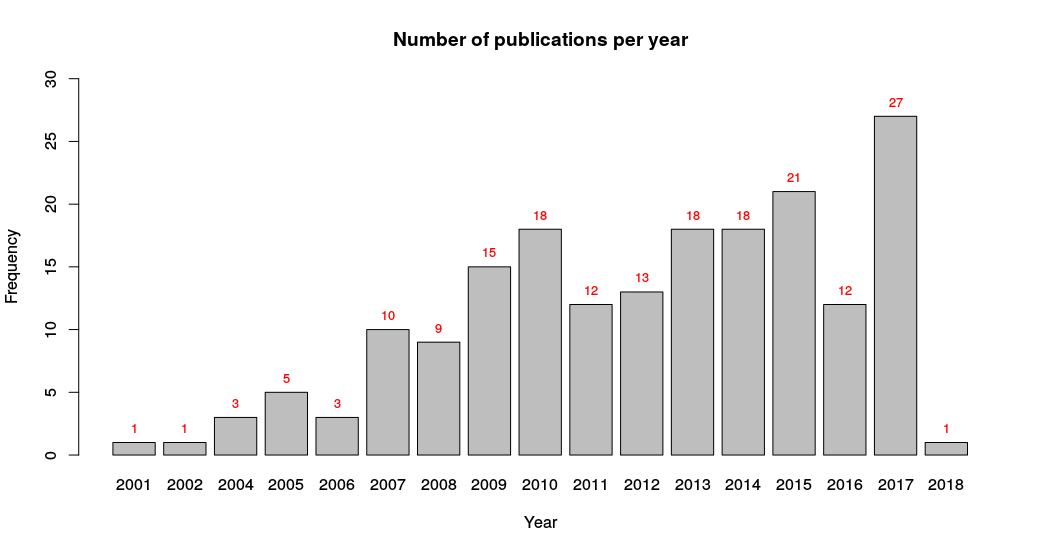
\includegraphics[width=\textwidth]{plots/Rplot.png}
%\caption{Results of inclusion phase}
%\end{figure}

\begin{figure}[ht]
\centering
\setlength\figureheight{7cm}
\setlength\figurewidth{\textwidth}
\input{plots/liter_rev/paper_distribution.tikz}
\caption{Distribution of papers per year after the inclusion phase.}
\end{figure}

After the inclusive search, we performed exclusion phase. This was done by filtering out manually all articles that were any of the following types: a review of certain aspect of source code plagiarism \eg student motives behind plagiarism, an improvement to some pre-existing algorithm \eg algorithmic speedups, plugin to online learning management systems, application to competition where the used method wasn't explained, study that used either byte-level information or information gathered during running the program, hashing techniques \eg compression and using the remaining size as a metric, system review which didn't address the method and theses. Beside these attributes, articles needed to also test their proposed method in some way and the amount of documents in experiment phase needed to be larger than two. The reason for adding this as a limiting factor was to gather studies that used test sets to evaluate the performance of their model.

The final number of articles after exclusion, and which are inspected more carefully in this systematic literature review is 32. From the set of 32 studies, we look answers for following questions: \emph{how plagiarism can be detected from source code}, \emph{what are possible features that can be derived from source code} and \emph{how can one identify the author of a given source code}. We start first by categorizing the articles by their themes to see what kind of different approaches there are to deal with the problem of plagiarism detection. After the initial classification, we summarize statistics about the data and briefly explain the used methods.


\subsection{Categorization}

The naïve categorization between articles can be done in a similar fashion as our query was constructed; dividing papers either to be about the detection of plagiarism or identifying the author of a given source code. However, as authorship identifying can also work as a way to detect plagiarism by verifying the author, we use the following high-level split visible in a table \ref{table-highcateq} where similarity detection is used as a second major category to avoid overlap.

\begin{table}[ht]
    \caption{Papers divided into two high-level categories}
    \label{table-highcateq}
    \centering
    \begin{tabular}{ | c | c | }
        
        \hline
        {\bf Similarity detection} & {\bf Authorship identification} \\ \hline
    
        \cite{AFAPLI2015, LICD2010, AASCPD2012} & \cite{SCAANN2017, ABEC2014, CAPSCAP2014}   \\
        \cite{Heblikar2015NormalizationBS, USCR2014, AIR2015} &  \cite{SCANG2007, EJPFSAI2004, ACSBPD2012}\\
        \cite{OTIOLSS2015, BUAA2009, ramirez2015high} &  \cite{APASCAI2007, UCMHGAAI2007, ESHPFSCAC2008}\\
        \cite{Ohmann2015, TBCFPD2012, Fu2017WASTKAW} &  \cite{AIRTSCAA2009, TSUDIJSCAI2011, DNNSCAI2013} \\
        \cite{ASTMLPD2013, AAPSCDPTK2013, CPDPPD2013}    & \cite{SCAIUFL2013, SDNAIJSP2015, AISC2017} \\
        \cite{PACASCD2005, RCISCP2017} &  \\ \hline
        {\bf Number of papers} & {\bf Number of papers} \\ \hline
        17 & 15 \\ \hline
    \end{tabular}
\end{table}

\noindent
Even though the articles are quite evenly divided in table \ref{table-highcateq}, these high-level groups are still too large to get a good overview of various methods. Thus we continue to categorize both groups into smaller atomic categorization, which reveals differences between and inside of them.  

Similarity detection in itself can be further divided into at least two general categories based on the current tools \cite{RSCAD2016}: attribute and structure. Then naturally, as authorship identification uses features derived directly from the source code too, we can use the same categorization to authorship identification studies. However, there are more finer categorizations that define the studies better based on the features they use, and thus we propose the following categories and their abbreviations: \emph{attribute counting (AC)}, \emph{segment matching (SM)}, \emph{n-gram (NG-STR)}, \emph{tree-based (TREE-STR)} and lastly \emph{hybrid approaches (HYB-STR)}. If a category has no studies under it, we leave the category out from the upcoming tables. These categories can be summarized briefly as following and are similar to categories identified from other plagiarism detection studies by Ali \etal \cite{OCPOCP2011}. 

\paragraph{Attribute counting}
Studies utilizing countable statistics, often referred as \emph{metrics}, that are gathered from source codes. This includes any features derived directly from source code like amount of words per line, number of lines per source code and number of keywords. For example the first two programs in appendix \ref{appendix:programs} represented as metrics is seen below.

\begin{table}[ht]
    \centering
    \begin{tabular}{|c|c|c|} \hline
        \textbf{Line count} & \textbf{Empty spaces} & \textbf{Semicolon count}\\ \hline
         10 & 1 & 5 \\ \hline
         8 & 1 & 3\\ \hline
    \end{tabular}
    \caption{First two programs in Appendix \ref{appendix:programs}; A and B represented as software metrics.}
    \label{tab:my_label}
\end{table}

\paragraph{Segment matching}
Considers two source codes as two strings and counts maximum match between them i.e. the longest common subsequence. These problems are also known as string matching problems, where one of the most famous algorithms is \emph{Greedy String Tiling} introduced early in \cite{SSGST1993}. As an example, statements \texttt{int a = 2;} and \texttt{int b = 2;} share 75\% of the character sequences and these matching sequences are: "\texttt{int}" and "\texttt{= 2;}". We also count all string similarity measures like string edit distances  to this category.

\paragraph{$N$-gram}
Treating the source code as a string and splitting it using a sliding window where the window size is the value of $n$ and the window traverses on either word or character level. This forms the vocabulary of the source code which is then transformed into occurrences of particular terms that are present, thus ultimately creating a vector representation of the source code. For example the statement \texttt{int a = 2} could be transformed into following word level 2-tuples using two as the value of $n$ (bigram). The first value of the following tuples is the $n$-gram extracted and the second value is the frequency: (\texttt{int a}, 1), (\texttt{a =}, 1), (\texttt{= 2}, 1). 

\paragraph{Tree-based}
Constructing a tree presentation from the source code, that captures the structure. For example diagram \ref{diag-parse} captures the structure of a simple assignment in parse tree, and one could compare \eg nodes of trees to define a similarity. The generation of a tree presentation usually requires some kind of parser being a very language specific feature. The inspection of a generated tree can be done with tree traversal methods for example using recursive functions. 

\paragraph{Hybrid}
Combines the usage of tree structure with $n$-gram representation. For example it can be a method which traverses abstract syntax tree, prints it and generates $n$-gram representation from the output.
\\\\
Now we can make a subcategorization for previously mentioned high-level classes; similarity detection and for authorship identification. Results for similarity detection studies can be seen from the following table, where most of them use structural features, indicated by the STR-ending. Many articles also tends to use $n$-grams to represent the source code.


\begin{table}[ht]
    \caption{Subgroups and sizes of similarity detection studies}
    \label{table-sdstudies}
    \centering
    \begin{tabular}{ | c | c | c | c | c |}
        
        \hline
        {\bf AC} & {\bf SM} & {\bf NG-STR} & {\bf AST-STR} & {\bf HYB-STR} \\ \hline
        \cite{PACASCD2005} & 
        \cite{LICD2010, ASTMLPD2013} & 
        \cite{AASCPD2012, USCR2014, AFAPLI2015} & 
        \cite{TBCFPD2012, AAPSCDPTK2013, AIR2015} & 
        \cite{BUAA2009, CPDPPD2013, RCISCP2017} \\
        & 
        & 
        \cite{Heblikar2015NormalizationBS, Ohmann2015, OTIOLSS2015} & 
        \cite{Fu2017WASTKAW} &
        \\
        & & \cite{ramirez2015high} &  & \\ \hline
        {\bf \#AC} & {\bf \#SM} & \multicolumn{3}{c |}{\bf \#STR} \\ \hline
        1 & 2 & \multicolumn{3}{c |}{14}
        \\ \hline
    \end{tabular}
\end{table}

When making the division for authorship studies, we can that in table \ref{table-aistudies} it is more evenly distributed in contrast to similarity detection articles in table \ref{table-sdstudies}. More studies now seem to utilize more countable attributes from source codes, but $n$-grams are as popular as they are in similarity detection. 

%, which is quite obvious when one considers that these methods are able to capture the writing style of an author from high-level features. For example authors can name the identifiers how they like, introduce comments and use various stylistic techniques when they write source code. 

\begin{table}[ht]
    \caption{Subgroups and sizes of authorship identification studies}
    \label{table-aistudies}
    \centering
    \begin{tabular}{ | c | c | c | c |}
        
        \hline
        {\bf AC} & {\bf NG-STR} & {\bf AST-STR} & {\bf HYB-STR} \\ \hline
        \cite{EJPFSAI2004, UCMHGAAI2007, APASCAI2007} & \cite{SCANG2007, ESHPFSCAC2008, AIRTSCAA2009} & \cite{SCAANN2017} & \cite{SDNAIJSP2015, AISC2017}\\ 
        \cite{ACSBPD2012, SCAIUFL2013, DNNSCAI2013} & \cite{TSUDIJSCAI2011, CAPSCAP2014, ABEC2014} & &\\ \hline
        {\bf \#AC} & \multicolumn{3}{c |}{\bf \#STR} \\ \hline
        6 & \multicolumn{3}{c |}{9}
        \\ \hline
    \end{tabular}
\end{table}

Results seems to show that utilizing structure is popular in both high-level classes, but quite dominant in similarity detection. Also both groups seems to show high popularity to the usage of $n$-grams, and interestingly authorship identification prefers to represent documents as statistical metrics.


\subsection{Descriptive statistics} \label{subsec-liter-data}
The data used in testing phase of 34 gathered studies is presented next, where the focus is for the similarity detection on following attributes: number of total documents, is there any synthetic data used and the average number of lines of code (Avg. LOC). For the authorship identification we focus on features like documents per author and number of possible authors. The term \emph{document} here refers to the number of source code file samples per author. We summarize the findings from data utilizing the categorization that was made earlier.

\paragraph{Similarity Detection}\mbox{}\\
Attribute counting study by Moussiades and Vakali in \cite{PACASCD2005} uses two real data sets written in C\texttt{++}. They contain programming assignments and a forged set of programs. The first data set contains 24 programs having an average of 247 lines of code per submission, the second set is 51 programs having an average of 178 lines per source code. The forged data set is two modified versions from one program, trying to deliberately confuse state-of-the-art detectors.

Segment matching study by Brixtel et al. used three corpora on their evaluation and are written in Haskell, Python and C \cite{LICD2010}. Haskell corpus had 13 documents averaging 400 lines per each, Python 15 documents averaging 150 lines per each and C 19 documents averaging 250 lines per source code. Study by Zhang and Liu used 12 programs written in C that all reflected different plagiarism strategies \cite{ASTMLPD2013}. 

Studies utilizing $n$-grams are summarized into following table.

\begin{table}[ht]
\centering
\caption{Data used in similarity detection studies utilizing $n$-grams}
\label{table-ng-str-data}
\begin{tabular}{|c|c|c|c|c|c|c|c|}
          \hline
          \backslashbox{\bf Feature}{\bf Paper} & \cite{AASCPD2012} & \cite{USCR2014} & \cite{AFAPLI2015} & \cite{Heblikar2015NormalizationBS} & \cite{Ohmann2015} & \cite{OTIOLSS2015} & \cite{ramirez2015high} \\ \hline
\bf Documents  &  179  & 5302   & 191  & 1356  & 2935  & 5408  & 1277   \\ \hline
\bf Synthetic &  No  & No  &  No  & No  & No  &  No & No  \\ \hline
\bf Avg. LOC & NA  & NA  & NA  & NA & NA  & 63.7  & NA  \\ \hline
\end{tabular}
\end{table}

\newpage

\noindent
It's visible from the table \ref{table-ng-str-data} that there are now a lot more documents used in experimentation and surprisingly synthetic data is not used at all. This is due to the usage of student submissions and competition data sets like \emph{Google Code Jam} submissions, which was for example utilized by Flores \etal in \cite{USCR2014}. 


\begin{table}[ht]
\centering
\caption{Data used in similarity detection studies utilizing abstract syntax tree}
\label{table-ast-str-data}
\begin{tabular}{|c|c|c|c|c|}
          \hline
          \backslashbox{\bf Feature}{\bf Paper} & \cite{TBCFPD2012} & \cite{AAPSCDPTK2013} & \cite{AIR2015} & \cite{Fu2017WASTKAW}\\ \hline
\bf Documents & 121 & 555 & NA & 22\,214  \\ \hline
\bf Synthetic & NA & No  & NA & Yes\\ \hline
\bf Avg. LOC & NA & 305.7 & NA & 20\\ \hline
\end{tabular}
\end{table}

\noindent
One can see from the table \ref{table-ast-str-data} that a study done by Fu \etal in \cite{Fu2017WASTKAW} has a large number of documents, and this due to two facts: they reported the size as pairs of documents and they used a generator to form a lot of forged documents from a small set of 10 original submissions. Ganguly and Jones in \cite{AIR2015} don't explicitly report the statistics of their data set, but refers to a competition test set called \emph{SOurce COde Re-use} (SOCO). This competition offers a set of C and Java files which contains known cases of cross-lingual plagiarism \cite{Flores:2014:DSC:2824864.2824878}. The train set size of SOCO is 338 files. 

Finally, hybrid study by Xiong \etal utilizes 40 assignments gathered from students \cite{BUAA2009}, Muddu \etal uses 5054 original files that they mutate to introduce copied code \cite{CPDPPD2013} and Ganguly \etal uses both train and test set of the SOCO competition, totaling around 12\,000 files \cite{RCISCP2017}. 


\paragraph{Authorship identification}\mbox{}\\
Usage of data in studies dealing with the problem of identifying the author and utilizing attribute counting are summarized to the following table, where we now turn the focus on the amount of candidate authors and documents per author reported in studies.

\begin{table}[ht]
\centering
\caption{Data used in authorship studies utilizing attribute counting}
\label{table-ai-ac-str-data}
\scalebox{0.9}{
    \begin{tabular}{|c|c|c|c|c|c|c|c|c|}
              \hline
              \backslashbox{\bf Feature}{\bf Paper} & \cite{EJPFSAI2004} & \cite{UCMHGAAI2007} & \cite{APASCAI2007} & (\cite{RA:AE2010}) & \cite{ACSBPD2012} & \cite{SCAIUFL2013} & \cite{DNNSCAI2013}\\ \hline
    \bf Authors  & 46 & 20 & 8 & 15 & 120 & 10 & 10 \\ \hline
    \bf Documents per author  & NA & 3 & 3 & 4 & NA & 61-377 & 61-377\\ \hline
    \bf Synthetic  & No & No & No & No & No & No & No\\ \hline
    \end{tabular}
}
\end{table}

\noindent
In table \ref{table-ai-ac-str-data}, one can see that there are two same data sets used in \cite{SCAIUFL2013, DNNSCAI2013}. This set was collected from \emph{SourceForge}\footnote{\url{https://sourceforge.net/}} projects and there are around 61 to 377 files per author. Rest of the attribute counting studies prefers to use \eg submissions gathered from students, as it's an easy way to gather tagged source code files.  

Next, data sets from the second popular method $n$-grams used in authorship identification, are summarized into following table.

\begin{table}[ht]
\centering
\caption{Data used in authorship studies utilizing $n$-grams}
\label{table-ai-ng-str-data}
    \begin{tabular}{|c|c|c|c|c|c|c|}
              \hline
              \backslashbox{\bf Feature}{\bf Paper} & \cite{SCANG2007} & \cite{ESHPFSCAC2008} & \cite{AIRTSCAA2009} & \cite{TSUDIJSCAI2011} & \cite{CAPSCAP2014} & \cite{ABEC2014}\\ \hline
    \bf Authors  & 100 & 8 & 100 & 8 & 30 & 30\\ \hline
    \bf Documents per author  & 14 & 2 & 14-26 & 2 & NA & NA\\ \hline
    \bf Synthetic  & No & No & No & No & No & No\\ \hline
    \end{tabular}
\end{table}

\noindent
There exists three different data sets used by three different authors in table \ref{table-ai-ng-str-data}: Burrows \etal in \cite{SCANG2007, AIRTSCAA2009} used data set gathered from students C programming assignments, Frantzeskou \etal in \cite{ESHPFSCAC2008, TSUDIJSCAI2011} used open-source programs written in Java and Tennyson \etal in \cite{CAPSCAP2014, ABEC2014} used programs written in \cpp and Java which mixture of were open-source, sample and textbook programs.

The only study that mainly used abstract syntax tree in their authorship study is by Alsulami \etal in \cite{SCAANN2017}. They used \emph{Google Code Jam} to gather 700 Python source code files belonging to 70 programmers averaging around 10 submissions per author. 

Finally, the data used in two hybrid studies are summarized. Wisse and Veenman used repositories from version control website called \emph{GitHub} \cite{SDNAIJSP2015}. The largest author pool they had while testing was 30. Zhang \etal had the data set also gathered from websites like \emph{GitHub} in their study \cite{AISC2017}. Their largest data set with respect to the author size, was imbalanced set of 503 programs belonging to 53 authors. 

\paragraph{Summary}\mbox{}\\
When looking the data usage of plagiarism study as a whole, one can see that almost all studies use data that is non-synthetic \ie use real-life data, that can be gathered for example from students course submissions or from competitions like SOCO. In similarity detection studies the median of the amount of source codes used is 447 and very few studies reported the average lines of code, which is a bit problematic as it can be easier to find plagiarism from a small set of program lines than from larger programs. In authorship attribution the median of possible authors in studies is 30 and the documents per author ranges from two to as high as 377.

% tarkista mediaani

\subsection{Methods} \label{chap-liter-review-methods}
In this chapter we turn the focus to the actual methods used in various studies. We use the same 
classification as a baseline for studies that was made earlier. The math used in studies is generalized to match the style of this paper, which means that a document is represented as $d$, matrices are bold and upper-cased $\bolditt{A}$, vectors are bold but lower-cased $\bolditt{a}$, tree structures $T$ and segments of source codes $S$ often implying strings. 

\paragraph{Similarity detection}\mbox{}\\
As a recap, the problem of similarity detection can be described formally as following.

\newtheorem*{smd}{Similarity detection}

\begin{smd}
Given a set of source code documents $D = \{d_1,...,d_n\}$, define similarity function $sim: d_i, d_j \rightarrow [0, 1]$ such that $sim(d_i, d_j) = sim(d_j, d_i)$ and $sim(d_i, d_i) = 1$, with a optional threshold $\theta \in [0, 1]$ that defines the limit where two source codes are considered as too similar. With this definition, any pair of source code file $(d_i, d_j) \in D \times D$ can also be presented as a triplet $(d_i, d_j, s)$, where $i \neq j$ and $s$ is the similarity value between documents. 
\end{smd}

The attribute counting study by Moussiades and Vakali uses a graph clustering on top of pair-wise similarities calculated using the Jaccard coefficient \cite{PACASCD2005}. Authors use following form of Jaccard coeficcient in their study where $A$ is the indexed set of substitute keywords per source code 

\begin{equation}\label{jacc_eqn}
    sim(d_1, d_2) = \dfrac{|A(d_1) \cap A(d_2)|}{|A(d_1) \cup A(d_2)|}
\end{equation}
\noindent
% refer to plag. attack
The indexed set can be built considering language dependent keywords \eg \texttt{while, for, false and true} in \cpp, and marking their position with respect to the occurrences of same keywords previously. However, authors claim that to generalize the set more, substitution keywords should be used. This means that for example all occurrences of \texttt{for}- and \texttt{while} -loops should be counted together, which helps to protect against plagiarism attack. The graph clustering algorithm Moussiades and Vakali uses is called \emph{WMajorClust} which works by presenting all pairs of source codes as non-directed graph $G = (V, E)$ where the set of vertices $V$ represents the source codes while the set of edges $E$ are weighted by equation \ref{jacc_eqn}. We can also express the definition of $E$ by Moussiades and Vakali with following constraints

\begin{equation}\label{jacc_edges_eqn}
         E = \Big\{ \{ d_i, d_j, sim(d_i, d_j)\} \, | \, (d_i, d_j) \in D \times D \land sim(d_i, d_j) \geq \theta \Big\}
\end{equation}

\noindent
%chapter ref
In equation \ref{jacc_edges_eqn}, $\theta$ is a user-defined parameter and works as a minimum threshold value that separates non-plagiarized source codes from plagiarized ones \ie two source codes will not share an edge if their similarity is below $\theta$.

Segment matching study by Brixtel \etal presents their algorithm, which builds from three major steps \cite{LICD2010}: pre-filtering, segmentation and document distance calculation. Their pre-filtering is to normalize the source code in a way, that every keyword and parameter definitions is transformed into a single symbol. As a segmentation, authors split the source code by lines forming set of segments $S_k$ presenting the partitioned set of a single source code. Similarity calculation happens by first forming distance matrix $\bolditt{M}$ between two source codes $d_1, d_2$ and then comparing all pairs of segments $(s_i^1, s_j^2) \in S_1 \times S_2$ where $S_k = (s_1^k, ..., s_n^k)$, with \emph{Levenshtein edit distance}. Distance matrix $\bolditt{M}$ is then transformed into noise reduction matrix $\bolditt{H}$ by finding the maximal matching between segmentations. Finally, $\bolditt{H}$ is filtered into a matrix $\bolditt{P}$ by convolution and utilizing a threshold\footnote{Authors used $\theta = 0.7$}. With the matrix $\bolditt{P}$, distance between two pairs of documents can be calculated by Brixtel \etal as 

\begin{equation}
    sim(d_1, d_2) = 1 - \dfrac{1}{\min(|S_1|, |S_2|)}\sum_{i, j} 1 - \bolditt{P}_{(i, j)}
\end{equation}

\noindent
Zhang and Liu utilize AST-tree and their core method is mainly constructed from two methods \cite{ASTMLPD2013}: forming the AST-representation and similarity calculation. Their AST-representation is done by traversing the parsed AST-tree and turning it into textual format by printing the nodes, and similarity calculation is computed using \emph{Smith Waterman algorithm} that finds the optimal matching between two strings $S_1, S_2$. Zhang et Liu gives the formula for similarity calculation between two source codes as

\begin{equation}
    sim(d_1, d_2) = \dfrac{2 \cdot \text{ SLength}(d_1, d_2)}{|S_1| + |S_2|}
\end{equation}
\noindent
Where SLength is the length of maximal matching string obtained via  \emph{Smith Waterman algorithm}, and $|S_k|$ represents the character length of one segment. 


$N$-gram studies take a different approach. Cosma and Joy uses \emph{Latent Semantic Analysis} to find suspicious documents \cite{AASCPD2012}. They first preprocess the documents by removing \eg short terms and comments. Then all documents are first transformed into a term-by-file matrix $\bolditt{A}$, where each document is represented as a occurrences of each unique term, which is same as forming the unigrams of a document. Values of $\bolditt{A}$ are weighted, and then $\bolditt{A}$ is decomposed via \emph{singular value decomposition} into $\bolditt{A} = \bolditt{U}\mathbf{\Sigma}\bolditt{V}^\intercal$ where $\bolditt{U}$ represents terms by dimension, $\mathbf{\Sigma}$ singular values and $\bolditt{V}$ files by dimensions. The dimensionality reduction is performed for all these matrices by considering only the first 30 columns. Finally, the similarity between a query vector $\bolditt{q}$ representing term frequency of document $d_i$, and document $d_j$ represented as a column $\bolditt{a}_j$ of matrix $\bolditt{A}$ is calculated by \emph{cosine similarity} \cite{AASCPD2012}

\begin{equation}\label{cosine_sim_eqn}
    sim(\bolditt{q}, d_j) = \cos \Theta_j = \dfrac{\bolditt{a}_j^\intercal \bolditt{q}}{\norm{\bolditt{a}_j}_2 \norm{\bolditt{q}}_2} = \dfrac{\bolditt{a}_j \boldsymbol{\cdot} \bolditt{q}}{\sqrt{\sum \limits_{i} \bolditt{a}_{(j, i)}^2} \sqrt{\sum \limits_{i} \bolditt{q}_i^2}}
\end{equation}

\noindent
Acampora and Cosma \cite{AFAPLI2015} continues on same style as Cosma and Joy \cite{AASCPD2012}, first preprocessing the documents by lowercasing and removing comments, syntactical tokens and short terms. Then using singular value decomposition with weighting to form three matrices from the corpus of source codes. For the reduced matrix $\bolditt{V}$ however, they perform a \emph{Fuzzy C-Means} clustering algorithm, which is tuned with \emph{ANFIS} learning algorithm to optimize the hyperparameters of Fuzzy C-means \cite{AFAPLI2015}. The process returns a membership degree $\mu_{i, k}$ per document, indicating how close $i$th document is to $k$th cluster. 
\noindent
Flores \etal \cite{USCR2014} uses similar preprocessing approach to Cosma and Joy. They first process the documents by lower-casing them and removing repeated character, tabs with spaces. Then transform the documents into $3$-grams and weighting them by using a \emph{term frequency}. Finally, similarity is calculated using cosine similarity where $t$ is one of the 3-grams and $tf$ is the term frequency function \cite{USCR2014}. Formally this can be calculated in a same way as in equation \ref{cosine_sim_eqn} between two documents as

\begin{equation}
    sim(d_i, d_j) = \dfrac{\sum\limits_{t \in d_i \cap d_j} tf(t, d_i) tf(t, d_j) }
                          {\sqrt{\sum\limits_{t \in d_i} tf(t, d_i)^2 \sum\limits_{t \in d_j} tf(t, d_j)^2}}
\end{equation}

\noindent
Heblikar \etal \cite{Heblikar2015NormalizationBS} preprocesses also their documents by lower-casing, pruning repeated whitespace and removing single symbols. They then normalize the documents by considering most frequent terms, renaming similar terms under same symbols and ultimately filtering them completely out from the source codes. For detection phase, they use same approach as Flores \etal did in \cite{USCR2014} but use both 1-grams and 2-grams with \emph{term frequency - inverse document frequency} (tf-idf) weighting. Interestingly, also Ramírez-de-la-Cruz \etal in \cite{OTIOLSS2015} and Ramírez-de-la-Cruz \etal in \cite{ramirez2015high} decides to use cosine similarity and Jaccard coefficient. The only major difference being, that Ramírez-de-la-Cruz \etal uses additional structural and stylistic features, forming total combination of eight various similarity measurements \cite{OTIOLSS2015}. Where as Ramírez-de-la-Cruz \etal in \cite{ramirez2015high} uses cosine similarity with character 3-grams to calculate five different similarities: lexical, stylistic, comments, text\footnote{Referring here as any string passed in as an argument of a function} and structural. Lastly, Ohmann and Rahal proposes density-based clustering to form clusters of similar documents \cite{Ohmann2015}. Their similarity approach follows closely to other studies presented above: filtering and normalization as preprocessing, data format as word $n$-grams and similarity values gained by using cosine similarity. 

Tree-based studies mostly relies on calculating similarity between two tree structures $T_i, T_j$ obtained from the original documents $d_i, d_j$ by parsing them. For example Ng \etal first generate parse tree $T$ from the source code, then decompose the parse tree into subtrees $T' \subseteq T$ with respect to the functionality \eg imports are categorized together \cite{TBCFPD2012}. The similarity score is obtained by comparing trees with \emph{depth-first search} and summing the scores for all subtrees to form a score between documents. This similarity function between two documents can be expressed with the following definition where $simST$ is the similarity score between two subtrees obtained by comparing their nodes and tokens

\begin{equation}
    sim(d_i, d_j) = sim(T_i, T_j) = \dfrac{\sum\limits_{i, j}simST(T'_i, T'_j)}{10 \cdot |T'|} \cdot 100
\end{equation}

\noindent
Son \etal computes similarity value between two parse trees with a modified parse tree kernel, and argue that their kernel function is able to consider also the length of the document \cite{AAPSCDPTK2013}. They define the kernel function $k$ via recursive function $C$ where $n$ is the node of a subtree $T'$. Function $C$ finds a maximal similarity between two nodes thus authors calls it also as the \emph{maximum node value}  

\begin{equation}
    k(T_i, T_j) = \sum\limits_{n_i \in T'_i} \sum\limits_{n_j \in T'_j} C(n_i, n_j)
\end{equation}

\noindent
The actual similarity between documents can be calculated then via normalization \cite{AAPSCDPTK2013}

\begin{equation}\label{norm_kern_eqn}
    sim(d_i, d_j) = \dfrac{k(T_i, T_j)}{\sqrt{k(T_i, T_i) \cdot k(T_j, T_j)}}
\end{equation}

% C(n_i, n_j) &= \lambda \prod \limits_{k}^{nc(n_i)} \left( 1 + \max\limits_{ch \in ch_{n_j}} C(ch_k(n_i), ch)\right)

\noindent
Another study that utilizes kernel between tree structures is by Fu \etal \cite{Fu2017WASTKAW}. They first build abstract syntax tree from a source code by normalizing and weighting nodes with term frequency–inverse document frequency, then use a tree kernel to measure similarity. Their normalization happens by transforming every variable name, array size definition and indexing of an array into single unified symbol. Then, Fu \etal remove all leaf nodes with common symbols to reduce noise, for example round and curly brackets. Finally, applied kernel method measures the edit distance of the content of expression nodes and for others, it uses calculates the similarity of subtrees with respect to their structure. In simplified way, the kernel method authors use can be expressed as dot-product between the occurances of possible subtrees expressed as vector $\bolditt{h}$ \cite{Fu2017WASTKAW}

\begin{equation}
    k(T_i, T_j) = \bolditt{h}(T_i') \boldsymbol{\cdot} \bolditt{h}(T_j')
\end{equation}

\noindent
With this definition of kernel, the similarity score between two source codes is calculated by normalizing the kernel values, leading ultimately to equation \ref{norm_kern_eqn}, which is the same as cosine similarity \cite{Fu2017WASTKAW}. The last tree-based study is by Ganguly and Jones. They use information retrieval approach and treat every document as a \emph{pseudo-query} \cite{AIR2015}. Basically this means that every document is first parsed into abstract syntax tree, then nodes belonging to similar functionality are collected together and finally specific fields are gathered from this collection by ranking them. For example all class definitions are treated as one collection and from that collection, names of the classes are extracted as weighted terms for constructing the pseudo-query. Ganguly and Jones claims that their approach allows to differentiate usage of same string literals in different situations.

Hybrid study by Xiong \etal presents their system named \textit{BUAA AntiPlagiarism} which uses abstract syntax tree to generate $n$-grams \cite{BUAA2009}. They first run the code through optimizer that gets rid of unnecessary complexity, then turn the simplified code into AST-representation and prune the tree by for example removing variable names and constants. This pruned tree is lastly travelled in preorder fashion that turns the tree into string format and form $n$-grams from that representation. To calculate similarity between documents, Xiong \etal uses Jaccard coefficient, which was defined earlier in equation \ref{jacc_eqn}, but now between sets of $n$-grams. Muddu \etal continues on combining approaches and presents their system called Code Plagiarism Detection Platform (CPDP) \cite{CPDPPD2013}. CPDP detects plagiarism by first tokenizing the AST, then turning the generated token stream into $4$-grams to be used in querying the $m$ matching documents. Finding the most closest document happens by using string matching algorithm \emph{Karp-Rabin Greedy String Tiling}, with given $n$-grams from the set of $m$ matching documents. Finally, the last similarity detection study is from Ganguly \etal in \cite{RCISCP2017}. They also use information retrieval approach in similar fashion as they did in previous work \cite{AIR2015}, to tackle with the problem related to $n$-grams without AST-representation; false-positives and exhaustive pair-wise calculation. Their method consists of building again pseudo-query and ranked list of most matching documents, where pseudo-query is built from various fields gathered from AST, for example from values of strings. With $m$ most matching documents, Ganguly \etal retrieves three kinds of features from them: lexical (3-grams); structural like identifiers, function types, and data types; and 11 stylistic features like average term length.   

\paragraph{Authorship identification}\mbox{}\\
The problem of authorship identification is very different from similarity detection. Instead of trying to find a function to represent a numerical value as similarity between two source code to detect plagiarism, authorship identification aims to reveal the writer of a document. It's common in following studies that the identification happens in closed environment, implying that the author of every document is known beforehand and can only be someone from the predefined set of possible authors. This situation can be used as authenticating and methods can be evaluated as the ground truth is known.

\newtheorem*{aui}{Authorship identification}

\begin{aui}
Given a set of documents $D$, a set of authors $A$ and a function $f: D \rightarrow A$ that identifies the writer by assigning every source code document $d \in D$ to one author $a \in A$. Estimate $f$ with $\hat{f}$, a classifier that treats every document as a feature vector $\bolditt{x}$ and every known class as a vector $\bolditt{y}$. The predicted author $\hat{y}$ can be thus expressed with $\hat{f}(\bolditt{x}) = \hat{y}$.
\end{aui}

Ding's and Samadzadeh's study follows the typical method of attribute counting studies. Authors extract total of 56 metrics belonging to three classes \cite{EJPFSAI2004}: layout, style and structure. Their feature selection is done by using variance and correlation analysis, whereas classification is done with \emph{canonical discriminant analysis}. Lange and Mancoridis extract 18 mostly text-based metrics and use genetic algorithm to find out the best combination \cite{UCMHGAAI2007}. Their classification is done by constructing a histogram per feature for every developer and then calculating which of the histograms are most closest to the unknown source code. Kothari \etal uses very similar histogram-based technique but considers style metrics and character distributions, namely character level $4$-grams \cite{APASCAI2007}. To select the most matching features for a single author, Kothari \etal uses information entropy which uses the distributions to make probabilistic evaluations. To classify the author, their approach is to have a database of writer profiles, extract metrics from source code and calculate the likelihood which known writer is the author. Arabyarmohamady \etal uses programming style to identify an author \cite{ACSBPD2012}. They build a profile for every author by transforming the source code into a feature vector \ie fingerprint and compare it to database of profiles to choose the most closest author profile. Plagiarism clusters are created by comparing the similarity of each feature vector with \emph{Euclidean distance}, thus allowing the detect issues with authorships and reveal plagiarism cases. Bandara and Wijayarathna has nine metrics that they use to generate tokens and token frequencies \cite{SCAIUFL2013}. For example, one of their metrics is number of characters per line (LLC) and to tokenize it, one creates token for specific length $n$ (LLC$_n$) and calculates the frequencies. This distribution of tokens is input to learning process called \emph{sparse auto-encoder} that learns to encode the features with neural network. Weights of this neural network are used as features to \emph{logistic regression} which classifies the author to document. Finally, similar study by again Bandara and Wijayarathna, uses now full neural networks for the same task \cite{DNNSCAI2013}. They use the same nine metrics with tokenization to get distributions per metric, and use them as a input to their deep neural network to learn to predict author from features.

Authorship identification with $n$-grams mostly use a baseline method called \emph{The Source Code Author Profile (SCAP)} in our review \cite{ESHPFSCAC2008, TSUDIJSCAI2011, CAPSCAP2014, ABEC2014}. The idea of SCAP is following: all known source codes from author $a$ are concated into one text file, $n$-grams are generated and only $L$ most frequent are kept per author to generate a profile $P$. To decide the author of a source code $d$, one calculates how many $n$-grams does unknown profile $P_d$ has in common with pre-existing author profile $P_a$

\begin{equation}
    \hat{y} = \argmax_{a \in A} |P_a \cap P_d|
\end{equation}

\noindent
The first study that uses its own method is by Burrows and Tahaghoghi. They approach the problem with information retrieval technique and consider author and document as queries \cite{SCANG2007}. Normalizing the documents is done by keeping only operators and keywords, while $n$-grams are used to present one document as overlapping sequences. Ranking the documents to create ranked list, happens with a proposed measure called \emph{Author1}. Author1-measure scores the similarity between documents and a query, and is defined using term frequencies for both query $q$ and document $d$

\begin{equation}
    \text{Author1}(q, d) = \sum\limits_{t \in q \cup d} \dfrac{1}{\min(|tf(t, q) - tf(t, d)|, 0.5)}
\end{equation}

\noindent
Burrow \etal continues on the topic of information retrieval in another study, where they experiment on six additional features on top of 6-grams \cite{AIRTSCAA2009}: white space, operators, literals, keywords, input/output (I/O) and function names. Rest of the $n$-gram related studies lean towards the SCAP method, mostly using it as a baseline while trying to improve it. For example Frantzeskou \etal analyzes the contribution of four different high-level features when using SCAP \cite{ESHPFSCAC2008}. These features are comments, layout features like spacing, identifier names and keywords. In another study, Frantzeskou \etal continues to use SCAP, but now studying the significance of user-defined identifiers with four categories \cite{TSUDIJSCAI2011}: identifiers using basic data types like \texttt{int} for integers, class identifiers, method identifiers and using all identifiers defined by the author. Tennyson and Mitropoulos study first the best profile length $L$ for SCAP \cite{CAPSCAP2014} and in another study, use two Bayesian methods to build an ensemble \cite{ABEC2014}. This ensemble works by using SCAP and Burrows method as a baseline to decide the author of a document. If there exists disagreement between baseline models, probability theory is used to classify the author. These two Bayesian methods are \emph{Maximum a Posteriori} and \emph{Bayes Optimal Classifier}, and both of them calculate probability that author $a$ wrote the document $d$ given previous data.



\newpage
\paragraph{Summary}
%\begin{algorithm}[ht]
%\caption{See how easy it is to provide algorithms}
%\label{myFirstAlgorithm}
%\begin{algorithmic}
%\REQUIRE $a$
%\STATE $b = 0$
%\STATE $x \leftarrow 1:10$
%\FORALL{x}
%    \STATE $b = b+a$
%\ENDFOR
%\RETURN $b$
%\end{algorithmic}
%\end{algorithm}

%\subsubsection{Accuracies}
%\input{liter_review/accuracies.tex}


\section{Research Design}

We base our model in this thesis to a claim that building a two phase model can reduce the amount of false-positives found in source code plagiarism detection. False-positives are problematic, as it would mean an innocent author would be considered as a possible plagiarist, thus having too sensitive models introduces a lot of extra work. These two phases of our model are similarity detection and authorship identification, where both of them are able to define a set of authors; similarity detection reveals suspicious authors based on the file similarity and authorship identification predicts candidate authors for a document $d$. 

%pre-process documents, tokenize documents, exclude templates, calculate similarities and finding suspects using these similarity scores.

Both of our models are inspired by other studies presented in the literature review and combine the high-level approach used in many tools \cite{RSCAD2016}: preprocess, normalize, calculate metrics and predict. The generalization of the proposed model is given below.

\begin{algorithm}[ht]
\caption{Detecting plagiarism between a set of source code files}
\label{alg-toplvl}
\begin{algorithmic}

\Require Set of authors $A$
\Require Set of source code files $D$ written by various authors $\forall a \in A$
\Procedure{PLGdetect}{$A, D$}
   \State $D'\gets normalize(D)$
   \State $D'_{train}, D'_{test} \gets split(D')$
   \State $\mathcal{M} \gets train(A, D'_{train})$
   \State $A_{auth} \gets \mathcal{M}(D'_{test})$
   \State $A_{susp} \gets detectSim(A, D'_{test})$
   \State \textbf{return} $A_{auth} \cap A_{susp}$
\EndProcedure

\end{algorithmic}
\end{algorithm}

\noindent
In algorithm \ref{alg-toplvl}, the source codes are first normalized to reduce the noise caused by \eg comments and repeated whitespace. We train a supervised learning model $\mathcal{M}$ that is able to classify the author of a document. We retrieve the top $n$ predictions called a set of candidate authors $A_{auth}$ for a document $d$. Similarity detection is calculated for the same set of documents to find suspicious authors $A_{susp}$. The word \emph{suspicious} refers here to too similar documents that are written by different authors. Finally, intersection between candidate authors and suspicious authors is taken, to provide a set of possible plagiarists. Both parts of our model are validated against real-life tools; plagiarism detection is evaluated against JPlag \cite{prechelt2002finding} which has been used as a baseline model in a SOCO competition \cite{saez2014pan}, and authorship identification against SCAP method.

\subsection{Assumptions}

We mainly focus on academia and especially to programming courses that are offered by 
universities. Following four assumptions are defined to simplify the problem of plagiarism
detection by allowing us to concern only plagiarism that happens in a closed environment and within a closed set of documents. 

\paragraph{In-class plagiarism} Plagiarism has occured only inside a 
specific course implementation. Let $\mathcal{P}(A)$ be a powerset of students within offered courses in university. We are only interested about a set of students referred as authors $A$ attended in a specific course $c$ \ie a subset $A_c \subseteq \mathcal{P}(A), A_c \neq \emptyset$. The corpus $D_c$ is built by gathering every submission done by students $\forall a \in A_c$ and a set of documents belonging to individual student is defined as $D_a = \{d \mid d \in D_c, a = auth(d)\}$. 


\paragraph{Exercise focus} 
Let $E_c = \{e_1, e_2, ..., e_n\}$ be a set of exercises for a course $c$, then submissions for a single exercise is represented by a subset $D_{c,e} \subseteq D_c$. With this assumption, we focus the plagiarism detection to submissions done to a single exercise at a time \ie plagiarism can happen only between submissions to a single exercise.

\paragraph{Single author} 
Every source code $d \in D_c$ is assumed to have a single author $a = auth(d), a \in A_c$. This allows us to assume that every source code submissions is done as a individual work, and all results that suggests otherwise implies about the case of excessive collaboration. 

\paragraph{Plagiarism direction} 
Let a file $d_i$ be plagiarized from $d_j$ \ie $d_i \xrightarrow{plag} d_j$, we treat this as same as the opposite direction $d_i \xleftarrow{plag} d_j$, making the direction of plagiarism unimportant. Thus the goal of our model is to give a set suspicious authors given the file and the claimed author.

\paragraph{Expert interference}
We believe that no system can be accurate enough to autonomously accuse students about plagiarism. However, this is doable when some form of human judgment is added to the model. In principal this means that the model can make predictions about cases of plagiarisms which we call \emph{suspects}, but the human expert must make the \emph{allegation} of plagiarism based on the results and after questioning the students.  

\subsection{Data set}

Our model is aimed to the traditional MOOC setting which is for example used by  undergraduate-level programming courses \emph{Introduction to Programming} (OHPE) and \emph{Advanced course in Programming} (OHJA) in University of Helsinki. We use all three real-life data sets; students submissions done to both of latter courses during the implementation in fall 2016 and a train data from SOCO task from 2014. All source code files are written in Java programming language. 

To implement our model, we first use SOCO to train and evaluate our similarity detection model, then train and test authorship identification with OHPE and OHJA. Our proposed model is built based on these results and plagiarism is detected individually for both courses. The reason to use train set of SOCO for similarity detection, is simply that it's the only data set that contains fully labeled cases of plagiarism, but unfortunately contains only one file per author. OHPE and OHJA on the other hand, contains multiple files per author making author identification possible, but only a few \emph{known} cases of plagiarism. Therefore we make use of both sets and consider our model to be successful if it finds at least every known case of plagiarism from OHPE and OHJA.

% TODO: add references from laptop
\paragraph{Course overview}\mbox{}\\
As courses, OHPE and OHJA shares the same structure; students first register to automatic scoring system called \emph{Test My Code} (TMC) which also distributes the exercises as an plugin to \emph{NetBeans IDE}, then independently work during seven weeks by completing programming exercises within deadlines. Students earn one point per exercise depending if all tests were successfully passed and complete an exam at end of the course, which is a programming exam that ultimately decides if a student has at least learned the minimum level required. There are no mandatory lectures, thus students are able to earn credits by working individually without any physical attendance. Also the exam in fall 2016 was a home exam, meaning that students were able to do it individually wherever they wanted to. 

\paragraph{SOCO overview}\mbox{}\\
Source code reuse (SOCO) data is from a 2014 competition \emph{PAN@FIRE}, where two sets were given to detect monolingual source code re-use \cite{saez2014pan}. SOCO2014 offered a train and a test set for competitors, which contained files written in \cpp\, and Java by various authors. The train set contains the source code files and annotations which are made by three experts flagging which pairs are considered as plagiarism. Competitors were then asked to retrieve which pairs are plagiarized. For example pair $(d_i, d_j)$ refers that there exists plagiarism between these two files, and because the direction was completely ignored, it was sufficient to retrieve just the predicted pairs.

SOCO contains mainly submissions to a single exercise and couple of documents, that are transformed from C to Java. As only the plagiarized file pairs are annotated and SOCO has been used successfully used in other studies \cite{AIR2015, RCISCP2017, OTIOLSS2015, USCR2014}, we make a simplifying assumption that the train set of SOCO contains one file per one unique author and that all submissions are submitted for the same task. This won't affect negatively the performance of our proposed model, as similarity detection is not affected at all if there exists multiple tasks within a corpus. 



\paragraph{Corpus statistics}\mbox{}\\
We are going to focus to Java language, therefore we only use the Java-specific part of SOCO training set, but fully utilize OHPE and OHJA data sets due to a fact that they only contain Java files. Number of non-transformative steps has been made beforehand to form the upcoming corpora: 1) leave SOCO as it is, 2) add exams to both OHPE and OHJA, and 3) concatenate submission containing multiple files into one file. This allows us to handle only one file per submission and we also get the benefit of having exam submissions, which is something where plagiarism is absolutely not allowed. 

%As OHPE and OHJA are both real-life courses, we also include the exam which in OHPE is made out of four tasks and in OHJA out of three tasks. 

Descriptive statistics for all three collections without any textual preprocessing is given in table \ref{tbl-corporastats}, where ten different metrics are reported: number of total authors, exercises and documents; does the corpus contains synthetic data; means for documents per author, character count, lines of code (LOC) and expressions\footnote{We assume countable expressions to be the ones ending in a semicolon}; and lastly minimum and maximum line counts. We can see from the table \ref{tbl-corporastats}, that SOCO has the smallest amount of authors but the tasks are more complex indicated by the largest LOC, amount of expressions and character count. When comparing OHPE to OHJA, OHPE has relatively smaller submissions than OHJA, which is mostly due to OHPE having easier tasks due to being the introductory course where students are not expected to know anything about programming beforehand. OHPE also has the most largest document-to-author ratio (106) compared to SOCO (1) and OHJA (56), making it the most richest data set when it comes to having a large amount of submissions per author.  Comparing to other corpora presented in chapter \ref{subsec-liter-data}, our OHPE corpus is one of the largest with OHJA. They both have over four times as many authors than any of the corpora used in other studies.

\begin{table}[ht]
\centering
\caption{Descriptive statistics for the unprocessed corpora. Bold values represents maximum per metric.}
\label{tbl-corporastats}
\begin{tabular}{|c|c|c|c|} \hline
\backslashbox{\bf Feature}{\bf Corpus}   & SOCO & OHPE & OHJA\\  \hline
\textbf{Authors}         & 259 & \textbf{316} & 270   \\  \hline
\textbf{Exercises}       & 1 & \textbf{151} & 92     \\  \hline
\textbf{Documents}       & 259 & \textbf{33\,363} & 15\,196    \\  \hline
\textbf{Documents per author $\mu$} & 1 & \textbf{106} & 56\\ \hline
\textbf{Synthetic}       & Partly & No & No \\  \hline
\textbf{LOC $\min$}         & \textbf{12} & 1 & 1      \\  \hline
\textbf{LOC $\mu$}        & \textbf{149} & 44 & 109     \\  \hline
\textbf{LOC $\max$}         & \textbf{1696} & 679 & 637   \\  \hline
\textbf{Expression $\mu$}       & \textbf{63} & 17 & 38 \\ \hline
\textbf{Character $\mu$} & \textbf{3898} & 1139 & 2794   \\  \hline
\end{tabular}
\end{table}

\newpage

A problem however arises when average line count with respect to the exercises is visualized for both OHPE and OHJA. Figure \ref{fig-hists} visualizes this by histograms, where both bin sizes are set to 50. 


\begin{figure}[!h]
\centering
\captionsetup[subfigure]{justification=centering}

\begin{subfigure}{\textwidth}
    \setlength\figureheight{5cm}
    \setlength\figurewidth{\textwidth}
    \input{plots/ohpe_avgloc.tikz}
    \label{fig-ohpeavgloc}
\end{subfigure}

\begin{subfigure}{\textwidth}
  \setlength\figureheight{5cm}
    \setlength\figurewidth{\textwidth}
    \input{plots/ohja_avgloc.tikz}
    \label{fig-ohjaavgloc}
\end{subfigure}

\caption[Two histograms for corpora]{Histograms showing average line of count per exercise for OHPE (top) and OHJA (below)}
\label{fig-hists}
\end{figure}

\noindent
From figure \ref{fig-hists} we see that majority of the submissions for OHPE has under 50 lines of code. This creates an issue for plagiarism detection, as there exists tasks where the submission can only contain a few dozen lines meaning, that the similarities between solutions will be naturally high. 

Consider for example three programs presented in appendix \ref{appendix:programs}. Because the solution to the given task is very limited, the submissions will inevitably have similar solutions, questioning the very fact that can there even exist plagiarism in short tasks. To overcome this problem we filter out all tasks where average line count falls to first quartile \ie under the 25th percentile, which is 21.0 for OHPE and 54.5 for OHJA. We call these filtered out tasks as \emph{trivial tasks} \ie exercises which solution space is very restricted. The intuition behind our filtering is that one cannot simply find plagiarism from too simple exercises which includes given tasks like: printing \say{Hello World} (1st task of OHPE), calculating how many seconds are in a year (6th task of OHPE) or doing simple string concatenation (2nd task of OHJA). 


\newpage

\subsection{Document representation}


\begin{figure}[!h]
\centering
\setlength\figureheight{5cm}
\setlength\figurewidth{8cm}
\input{plots/fig.tikz}

\caption{TEST} \label{fig:M1}
\end{figure}

\subsection{Normalization}

\subsection{Similarity detection}

%use t-SNE for visualization!! density is lost https://stats.stackexchange.com/questions/263539/k-means-clustering-on-the-output-of-t-sne?utm_medium=organic&utm_source=google_rich_qa&utm_campaign=google_rich_qa

\subsection{Authorship identification}



\subsection{Evaluation metrics}

\section{Results}

Following chapters describe the results we gathered during the evaluation of our models. All results are generated using Python version 3.6.0\footnote{\url{https://www.python.org/} Accessed 14th May 2018} and scikit-learn version 0.19.1\footnote{\url{http://scikit-learn.org/stable/} Accessed 14th May 2018}. 

As explained in the Chapter \ref{chap-method-evaluation}, we first evaluate both models individually and lastly combine the results to create a final prediction which is evaluated by a human expert. Our similarity detection is trained with SOCO data set and authorship identification with OHPE and OHJA without using the exams. A summary of these exam tasks is given below.

\begin{table}[ht]
\centering
\caption{Submission count and average line count for exam tasks. A refers to OHPE and B for OHJA.}
\label{tbl-exam-data}
\begin{tabular}{|c||c|c|c|c|c|c|c|}
\hline
\bf Task        & 1.A & 2.A & 3.A & 4.A & 1.B & 2.B & 3.B \\ \hline
\bf Submissions & 244 & 242 & 227 & 240 & 200 & 198 & 197 \\ \hline
\bf Avg. LOC    & 37  & 39  & 47  & 110 & 160 & 86  & 150 \\ \hline
\end{tabular}
\end{table}

\noindent
It's clear from the Table \ref{tbl-exam-data} that OHJA's tasks are more longer than OHPE's. Some of the tasks of OHPE's exam have a very low average line count that creates a challenge for the detection.

\subsection{Document similarity} \label{chap-sd-result}
% macro-averaged results

We start evaluating our similarity detection by tuning the hyperparameters. Results are gained by turning all documents into binary vector based on the SOCO labels \ie vector $\bolditt{y}$ where $y_i = 1$ and $y_j = 1$ if $i$th and $j$th documents are reported as plagiarized pairs. Our predictions are then compared to this golden standard.

Following table shows averaged $F_1$-score for the SOCO-T data.  

\begin{table}[ht]
\centering
\caption{Average $F_1$-score for $n$-gram length and $\varepsilon$-range for SOCO-T. The smaller the $\varepsilon$-range is, the more similar documents have to be. $F_1$-scores close or over 0.8 are bolded.}
\label{tbl-sd-socot-fone}
\scalebox{0.75}{
    \begin{tabular}{|c||c|c|c|c|c|c|c|c|c|c|} \hline
    \backslashbox{\bf Epsilon}{\bf $N$-gram} & 1 & 2 & 3 & 4 & 5 & 6 & 7 & 8 & 9 & 10 \\ \hline
    0.1 & 0.31  & 0.69  & 0.63  & 0.60  & 0.59  & 0.56 & 0.55  & 0.55   & 0.52  & 0.52   \\ \hline
    
    0.2 & 0.28  & 0.59  & 0.73  & 0.66  & 0.63  &  0.62  & 0.60  & 0.59  & 0.56  &  0.55 \\\hline
    
    0.3 &  0.27  & 0.43  & \bf 0.78 & 0.73  & 0.70  & 0.67  & 0.64 & 0.63 & 0.59  & 0.58   \\ \hline
    
    0.4 & 0.27  & 0.31  & 0.72  & \bf 0.81  & \bf 0.78  & 0.72   &  0.71  & 0.69  & 0.65  & 0.64  \\ \hline
    
    0.5 & 0.27  & 0.29  & 0.57  & \bf 0.80  & \bf 0.81  & \bf 0.80  & \bf 0.81  & \bf 0.78 &  0.77   & 0.74   \\ \hline
    
    0.6 & 0.27  & 0.27  & 0.39  & 0.71  & \bf 0.83  & \bf 0.89  & \bf 0.90  &  \bf 0.86  & \bf 0.85 & \bf 0.85   \\ \hline
    
    \end{tabular}
}
\end{table}

\noindent
One can see from the Table \ref{tbl-sd-socot-fone} that for the training data of SOCO, the $F_1$-score is highest when $n \in [4, 7]$ and $\varepsilon \in [0.4, 0.6]$. However using 60\% similarity between 

Precision matrix for all hyperparameters SOCO:

\begin{table}[ht]
\centering
\caption{Precision for plagiarized documents ranging various $n$-gram lengths and $\varepsilon$-ranges for SOCO. Values close or over 0.9 are bolded.}
\label{tbl-sd-soco-prec}
\scalebox{0.75}{
    \begin{tabular}{|c||c|c|c|c|c|c|c|c|c|c|} \hline
    \backslashbox{\bf Epsilon}{\bf $n$-gram} 
        & 1 & 2 & 3 & 4 & 5 & 6 & 7 & 8 & 9 & 10 \\ \hline
    0.1 & 0.45  & 0.77  & \bf 1.00  & \bf 1.00  & \bf 1.00  & \bf 1.00 & \bf 1.00  & \bf 1.00   & \bf 1.00  & \bf 1.00   \\ \hline
    
    0.2 & 0.45  & 0.53  & \bf 0.98  & \bf 1.00  & \bf 1.00  &  \bf 1.00  & \bf 1.00  & \bf 1.00  & \bf 1.00  &  \bf 1.00 \\\hline
    
    0.3 &  0.44  & 0.48  &  0.83 & \bf 1.00  & \bf 1.00  & \bf 1.00  & \bf 1.00 & \bf 1.00 & \bf 1.00  & \bf 1.00  \\ \hline
    
    0.4 & 0.44  & 0.45  & 0.63  & \bf 0.87  & \bf 0.97  & \bf 0.98  &  \bf 0.98  & \bf 1.00  & \bf 1.00 & \bf 1.00  \\ \hline
    
    0.5 & 0.44  & 0.45  & 0.54  & 0.75  & \bf 0.90  &  \bf 0.92  &  \bf 0.97  & \bf 0.98 &  \bf 1.00   & \bf 1.00   \\ \hline
    
    0.6 & 0.44  & 0.44  & 0.47  & 0.62  & 0.77  & \bf 0.87  & \bf 0.94  & \bf 0.93  & \bf 0.95 & \bf 0.96   \\ \hline
    
    \end{tabular}
}
\end{table}

% The epsilon is large and n-grams long

We see from the Table \ref{tbl-sd-soco-prec}, that as we grow the number of $n$-grams, the precision converges to 1.00. This means that the set of retrieved documents contains high number of true-positives, as we have effectively minimized the amount of false-positives, meaning that no document is falsely accused of plagiarism. The most precise predictions are always when the epsilon is as low as 0.1 meaning that documents have to have 90\% of structural similarity. 

However, with a low epsilon value the precision for detecting plagiarized documents quickly lowers unless one grows the $n$-gram length. This can lead to problem of retrieving l 

\begin{table}[ht]
\centering
\caption{Average $F_1$-score for SOCO C1, which contains no plagiarism.}
\scalebox{0.75}{
    \begin{tabular}{|c||c|c|c|c|c|c|c|c|c|c|}
    \hline
    \backslashbox{\bf Epsilon}{\bf $n$-gram}    & 1    & 2    & 3    & 4    & 5    & 6    & 7    & 8    & 9    & 10   \\ \hline
    0.1 & 0.24 & \bf 0.94 & \bf 0.99 & \bf 0.99 & \bf 0.99 & \bf 0.99 & \bf 0.99 & \bf 0.99 & \bf 0.99 & \bf 0.99 \\ \hline
    0.2 & 0.11 & 0.56 & \bf 0.98 & \bf 0.99 & \bf 0.99 & \bf 0.99 & \bf 0.99 & \bf 0.99 & \bf 0.99 & \bf 0.99 \\ \hline
    0.3 & 0.06 & 0.38 & \bf 0.95 & \bf 0.99 & \bf 0.98 & \bf 0.99 & \bf 0.99 & \bf 0.99 & \bf 0.99 & \bf 0.99 \\ \hline
    0.4 & 0.03 & 0.20  & \bf 0.87 & \bf 0.98 & \bf 0.98 & \bf 0.98 & \bf 0.98 & \bf 0.98 & \bf 0.98 & \bf 0.98 \\ \hline
    0.5 & 0.03 & 0.16 & 0.59 & \bf 0.95 & \bf 0.98 & \bf 0.98 & \bf 0.98 & \bf 0.98 & \bf 0.98 & \bf 0.98 \\ \hline
    0.6 & 0.02 & 0.08 & 0.29 & \bf 0.88 & \bf 0.96 & \bf 0.98 & \bf 0.98 & \bf 0.98 & \bf 0.98 & \bf 0.98 \\ \hline
    \end{tabular}
}
\end{table}

\begin{table}[ht]
\centering
\caption{Average $F_1$-score for SOCO C2, which contains 28 cases of plagiarism.}
\scalebox{0.75}{
   \begin{tabular}{|c||c|c|c|c|c|c|c|c|c|c|}
    \hline
     \backslashbox{\bf Epsilon}{\bf $n$-gram}     & 1    & 2    & 3    & 4    & 5    & 6    & 7    & 8    & 9    & 10   \\ \hline
    0.1 & 0.34 & \bf 0.92 & \bf 1.00 & \bf 1.00 & \bf 1.00 & \bf 1.00 & \bf 1.00 & \bf 1.00 & \bf 1.00 & \bf 1.00 \\ \hline
    0.2 & 0.27 & 0.57 & \bf 1.00 & \bf 1.00 & \bf 1.00 & \bf 1.00 & \bf 1.00 & \bf 1.00 & \bf 1.00 & \bf 1.00 \\ \hline
    0.3 & 0.20 & 0.38 & \bf 0.92 & \bf 1.00 & \bf 1.00 & \bf 1.00 & \bf 1.00 & \bf 1.00 & \bf 1.00 & \bf 1.00 \\ \hline
    0.4 & 0.15 & 0.31 & 0.75 & \bf 0.97 & \bf 0.97 & \bf 0.99 & \bf 0.99 & \bf 0.99 & \bf 0.99 & \bf 1.00 \\ \hline
    0.5 & 0.15 & 0.27 & 0.47 & \bf 0.91 & \bf 0.97 & \bf 0.97 & \bf 0.97 & \bf 0.97 & \bf 0.99 & \bf 0.99 \\ \hline
    0.6 & 0.15 & 0.22 & 0.33 & 0.78 & \bf 0.92 & \bf 0.97 & \bf 0.97 & \bf 0.97 & \bf 0.97 & \bf 0.97 \\ \hline
    \end{tabular}
}
\end{table}

\newpage

Following table shows recall and accuracy of the best performing models with respect to $F_1$ and precision.

\begin{table}[ht]
\centering
\caption{Recall over positive classes (plagiarism).}
\label{lbl-sd-best-perf}
\begin{tabular}{|c|c|c|c|} \hline
$\varepsilon$  & $n$-gram & Recall & ACC  \\ \hhline{|=|=|=|=|}
0.4 & 4  & 0.68   & 0.81 \\ \hline
0.4 & 5  & 0.54   & 0.79 \\ 
0.5 & 5  & 0.67   & 0.82 \\ \hline
0.5 & 6  & 0.67   & 0.88 \\
0.6 & 6  & \bf 0.86   & 0.88 \\ \hline
0.5 & 7  & 0.60    & 0.81 \\
0.6 & 7  & 0.83   & \bf 0.90  \\ \hline
0.6 & 8  & 0.75   & 0.86 \\ \hline
0.6 & 9  & 0.71   & 0.86 \\ \hline
0.6 & 10 & 0.69   & 0.85 \\ \hline
\end{tabular}
\end{table}

Results show that $\varepsilon = 0.6$ and $n$-gram length six, seems to work for our model. 

Confusion matrix SD SOCO:

\begin{table}[ht]
\centering
\caption{Confusion matrix for best performing model (6-g)}
\label{tbl-sd-soco-conf}
\scalebox{1}{
    \begin{tabular}{l|c|c|c|c}
    \multicolumn{2}{c}{}&\multicolumn{2}{c}{True}&\\
    \cline{3-4}
    \multicolumn{2}{c|}{}&\bf Non-plagiarized& \bf Plagiarized\\
    \cline{2-4}
    \multirow{2}{*}{Predicted}& \bf Non-plagiarized & $129$ & $15$\\
    \cline{2-4}
    & \bf Plagiarized & $16$ & $99$ \\
    \cline{2-4}
    
    \end{tabular}
}
\end{table}



Following table shows metrics when JPlag is applied for SOCO. Average values over non-plagiarized and plagiarized classes are reported

\begin{table}[ht]
\centering
\caption{JPlag SOCO}
\label{tbl-jplag-soco}
\begin{tabular}{|c||c|c|c|c|c|c|} \hline
\bf Similarity threshold & 90\% & 80\% & 70\% & 60\% & 50\% & 40\% \\ \hline
\bf F1                  & 0.59   &  0.65   &  0.72   &  0.87   &  0.96   & \bf 0.97    \\ \hline
\bf Precision           & 0.79    &  0.80   &  0.83   &  0.90   & 0.96    &  \bf 0.97   \\ \hline
\bf Recall              &  0.66   &  0.69    &  0.75   & 0.88    &  0.96   & \bf 0.97     \\ \hline
\bf Accuracy            &  0.66   &  0.69   & 0.75    &  0.88   &  0.96   & \bf 0.97   \\ \hline
\end{tabular}
\end{table}

\newpage


Confusion matrix:

\begin{table}[ht]
\centering
\caption{Confusion matrix for the best performing JPlag (sim 40\%)}
\label{tbl-jplag-soco-conf}
\scalebox{1}{
    \begin{tabular}{l|c|c|c|c}
    \multicolumn{2}{c}{}&\multicolumn{2}{c}{True}&\\
    \cline{3-4}
    \multicolumn{2}{c|}{}&\bf Non-plagiarized& \bf Plagiarized\\
    \cline{2-4}
    \multirow{2}{*}{Predicted}& \bf Non-plagiarized & $136$ & $1$\\
    \cline{2-4}
    & \bf Plagiarized & $8$ & $114$ \\
    \cline{2-4}
    
    \end{tabular}
}
\end{table}

As we see from the confusion matrices, our similarity detection performs closely to the JPlag. To see how well our clusters agree with JPlag, we calculcate the Jaccard similarity between these two predictions. This agreement based on our model using 6-grams with $\varepsilon = 0.6$, and JPlag with 40\% similarity treshold is x.

!!!<SD(OHPE/OHJA) VS JPLAG JACCARD>!!!




\subsection{Authorship identification}
Our authorship identification model requires one parameter to be tuned, the length
of character-level $n$-grams to be extracted. We tune this parameter based on the average $F_1$-score and accuracy over seven split points for both OHPE and OHJA. For every weekly split the final exercise is left out as a test data, 80\% of the remaining data is used for training and 20\% for validation. The training data is used purely to tune the model, whereas validation is used to find the best performing $n$-gram length. After the value for $n$ has been found, we evaluate the final model with the test data. 

Tables below show the splits we make, the number of students submitted to the last exercise of the week and the average profile size. The profile size refers simply to the amount of documents students have submitted before the split.


\begin{table}[ht]
\centering
\caption{OHPE's splits. Profile size grows naturally as students progress the course.}
\label{lbl-result-ai-ohpe-stat}
\begin{tabular}{|c||c|c|c|c|c|c|c|}
\hline
\bf Week             & 1.   & 2.   & 3.   & 4.   & 5.   & 6.   & 7.   \\ \hline
\bf Students         & 230 & 239 & 189 & 174 & 127 & 138 & 53  \\ \hline
\bf AVG. Profile size & 24  & 40  & 64  & 76  & 85  & 94  & 102 \\ \hline
\end{tabular}
\end{table}

\begin{table}[ht]
\centering
\caption{OHJA's splits. The profile size is much lower than in OHPE.}
\label{lbl-result-ai-ohja-stat}
\begin{tabular}{|c||c|c|c|c|c|c|c|}
\hline
\bf Week             & 1.   & 2.   & 3.   & 4.  & 5.   & 6.   & 7.   \\ \hline
\bf Students         & 144 & 114 & 137 & 90 & 111 & 121 & 113 \\ \hline
\bf AVG. Profile size & 11  & 21  & 30  & 36 & 43  & 50  & 53  \\ \hline
\end{tabular}
\end{table}

\noindent
We see in Table \ref{lbl-result-ai-ohpe-stat} how the amount of students varies quite a bit for the final week as only 53 students submitted. This is probably because students have calculated that they already got the points they need in order to pass the course with the exam, so they skip the last exercise. The amount of students remains more stable in OHJA seen in Table \ref{lbl-result-ai-ohja-stat}, where the profile size grows more steadily. 

For every split in OHPE we calculated the macro-averaged $F_1$ for the validation data and got following results.


\begin{table}[ht]
\centering
\caption{Macro-averaged $F_1$-score calculated for each validation set of OHPE.}
\label{lbl-result-ai-f1-ohpe}
\def\arraystretch{1.5}
\begin{tabular}{|c|c|c|c|c|c|c|c|c|} \hline
\backslashbox{\bf $n$-gram}{\bf Week}  & 1. & 2. & 3. & 4. & 5. & 6. & 7. \\ \hline
2     & 0.01 & 0.02 & 0.03 & 0.02 & 0.02 & 0.02 & 0.03 \\ \hline
4     &     0.01 & 0.03  & 0.03  & 0.04  & 0.04  & 0.04  & 0.04    \\ \hline
6     &  0.02    & 0.04  & 0.05  & 0.05  & 0.05  & 0.05  & 0.05    \\ \hline
8     & 0.02     & 0.04  & 0.05  & 0.06  & 0.06  & 0.06  & 0.06    \\ \hline
10    &  0.02    & 0.05  & 0.06  & 0.06  & 0.07  & 0.07  & 0.07     \\ \hline
12    & 0.02     & 0.05  & 0.06  & 0.06  & 0.07  & 0.07  & 0.07     \\ \hline
14    & 0.02     & 0.05  & 0.06  & 0.07  & 0.07  & 0.07  & 0.07    \\ \hline
\end{tabular}
\end{table}

\noindent
Table \ref{lbl-result-ai-f1-ohpe} shows how the model fails to predict the correct authors in multiclass setting, where each document can be predicted only to one author. We see that the $F_1$-score slightly increases when $n \geq 10$ and when the used weeks grows \ie the submission amount per student grows. The same evaluation was also run for the OHJA, but the results were as poor as for the OHPE, and therefore they are not shown here. Based on these result we fix the $n$-gram length as 10, as it's the best overall result we got with the smallest $n$ used which also limits the size of vocabulary.

Figure \ref{fig-ai-ohpe-ngram-voc} reveals how the vocabulary size grows when the $n$-gram length gets larger. Even by using a small value of $n$ which keeps the vocabulary size smallest and should effectively capture \eg the spacing used after operator symbols, gives poor results as seen in Table \ref{lbl-result-ai-f1-ohpe}. However the problem with large vocabulary is that the training consists a lot of noisy features \ie features that could be dismissed completely, that the model is unable to find important features and weight them properly. 

\newpage

\begin{figure}[ht]
    \centering
    \setlength\figureheight{5cm}
    \setlength\figurewidth{0.8\textwidth}
    \input{plots/result/AI/n_gram_to_voca.tikz}
    \caption{Vocabulary size in $\log_{10}$-scale with respect to character $n$-gram length. Vocabulary is formed using 80\% of OHPE's tasks (training set) and its size for 10-grams is around 278\,000.}
    \label{fig-ai-ohpe-ngram-voc}
\end{figure}


As we look the ten most common $n$-grams formed from the training using OHPE's data set and their frequencies, we see how similar most of the features are from Table \ref{tbl-ai-result-topten-ngrams}. 

\begin{table}[ht]
    \centering
    \caption{Ten most frequent 10-grams encountered while training the Naïve Bayes model. All of them contain the same overlapping sequence which is the statement for printing in Java.}
    \begin{tabular}{|m{4cm}|l|}
    \hline
    \textbf{$N$-gram} & \textbf{Frequency} \\ \hline
    \texttt{System.out}     & 18643              \\ \hline
    \texttt{ystem.out.}     & 18643              \\ \hline
    \texttt{stem.out.p}     & 18643              \\ \hline
    \texttt{tem.out.pr}     & 18643              \\ \hline
    \texttt{em.out.pri}     & 18643              \\ \hline
    \texttt{m.out.prin}     & 18643              \\ \hline
    \texttt{.out.print}     & 18643              \\ \hline
    \texttt{System.ou}      & 18640              \\ \hline
   \texttt{out.printl}     & 15171              \\ \hline
    \texttt{ut.println}     & 15171              \\ \hline
    \end{tabular}
    \label{tbl-ai-result-topten-ngrams}
\end{table}

\noindent
In Table \ref{tbl-ai-result-topten-ngrams}, most of the programs contain various sequences of the same print statement in Java language. These statements exist in almost every document, as many of the tasks in OHPE and OHJA require to print various values to the console in order to evaluate the correctness of the submission. All of these  10-grams can be considered as noise, because their informative value is close to zero as they are used in similar way in all documents. Features like these are problematic for our identification because as the vocabulary size grows, the vector representing the document is starting to contain mostly zeroes and the non-zero ones can contain a lot of non-informative duplicates as are the 10-grams in Table \ref{tbl-ai-result-topten-ngrams}.

We looked would the data be skewed while training \ie would some author have a majority of the documents, giving untrue prior probabilities for authors. However this was not the case as seen from the following plot.

\begin{figure}[ht]
    \centering
    \setlength\figureheight{5.5cm}
    \setlength\figurewidth{\textwidth}
    \input{plots/result/AI/author_to_document_dist_ohpe.tikz}
    \caption{The profile size of each included author in OHPE's training set.}
    \label{fig-author-to-document-dist-ohpe}
\end{figure}

\noindent
There are only four authors 2, 35, 41 and 49 who are below the average profile size in Figure \ref{fig-author-to-document-dist-ohpe}, so we can't say that our data would have been skewed in the training process. The data is very evenly spread amongst the authors, as nearly all have around 100 documents for their profile size. When comparing these numbers to other studies presented during literature review in Chapter \ref{subsec-liter-data}, we see that not only we have around ten times more documents per authors, but also our author pool is a lot larger. Having a lot of sample documents for each author should generate more distinct writing preferences, but in our case it's not the case as submissions seem to be too similar. Excessive similarity was a problem also in our similarity detection evaluation in Chapter \ref{chap-sd-result}.


To see the missclassification of our model, we formed the frequencies of true authors and the predicted authors in the validation data of OHPE. Figure \ref{fig-ai-result-author-distr} shows how the authorship identification should produce a uniform distribution of authors, where each author has around 25 documents classified for them. However, our model can't find enough unique stylistic preferences during the training, thus misclassifying majority of the documents to four authors. This result reflects the same observation that was made earlier about the excessive similarity of the documents. The similarity between source code documents leads to situation where some amount of authors might be so close to other profiles, that there any not enough discriminating $n$-grams which could divide authors apart from each other. This problem is visualized in Figure \ref{fig-ai-result-author-distr} as spikes, where four authors become author archetypes who capture the same writing style as everybody else.

\newpage

\begin{figure}[ht] 
  \centering
  \begin{subfigure}[b]{\linewidth}
    \centering
    \setlength\figureheight{5.5cm}
    \setlength\figurewidth{\textwidth}
    \input{plots/result/AI/true_distr_ohpe_val_labels.tikz}
    \caption{True author distribution. The number of samples for each class in the validation data is averaging around 25, with just a few outliers.}
    \vspace{4ex}
  \end{subfigure}
  \begin{subfigure}[b]{\linewidth}
    \centering
    \setlength\figureheight{5.5cm}
    \setlength\figurewidth{\textwidth}
    \input{plots/result/AI/pred_distr_ohpe_val_labels.tikz}
    \caption{Predicted author distribution. There are several authors without any documents classified to them, and four authors who have the majority.}
  \end{subfigure}
  \caption{The true distribution of authors in the validation data of OHPE (a) compared to the predicted distribution (b). Our classifier predicts most of documents to belong to just four unique authors.}
  \label{fig-ai-result-author-distr}
\end{figure}



Inspecting the probabilities of the Multinomial Naïve Bayes which is trained with OHPE, the mean prior is 0.02 (2\%) and the standard deviation 0.002. This means that the prior probabilities $P(y)$ are very close to each other so their influence is diminished at the prediction phase. The likelihood \ie probability of the $i$th feature appearing given the class $P(x_i | y)$, is also very small for every feature and class combination, as using 10-grams there are around 246\,000 unique features. For every class the mean conditional probability is $4.1 \times 10^{-6}$ and standard deviations for conditional probabilities are in range $[1.3 \times 10^{-7}, 2.0 \times 10^{-7}]$, showing again how similar all values are because our vocabulary is too large. 

As we have now shown the results for training and validation, selected the $n$-gram length as 10 and looked some of the reasons why the model fails to predict the author, we next present the results for the test data. It consist of the last exercises and uses all possible data for the training phase, as shown in Table \ref{lbl-result-ai-ohpe-stat} and Table \ref{lbl-result-ai-ohja-stat}. We will restrict the author pool size to ease the problem and use the last week for both OHPE and OHJA to have a full data set, and these results for both $F_1$-score and accuracy are visible in Figure \ref{fig-ai-result-ohpeohja-testset}. 


\begin{figure}[!h] 
  \centering
  \begin{subfigure}[b]{\linewidth}
    \centering
    \setlength\figureheight{6cm}
    \setlength\figurewidth{\textwidth}
    \input{plots/result/AI/ohpeohja_f1_per_authorpool.tikz}
    \caption{$F_1$-score for OHPE's and OHJA's test set using 10-grams and varying the amount of possible authors.}
    \label{fig-ai-result-ohpeohja-testset:a}
    \vspace{4ex}
  \end{subfigure}
  \begin{subfigure}[b]{\linewidth}
    \centering
    \setlength\figureheight{6cm}
    \setlength\figurewidth{\textwidth}
    \input{plots/result/AI/ohpeohja_acc_per_authorpool.tikz}
    \caption{Accuracy for OHPE's and OHJA's test sets using 10-grams with various author pool sizes.}
  \label{fig-ai-result-ohpeohja-testset:b}
  \end{subfigure}
  \caption{Evaluation results for the final authorship identification model. Our model is not able to predict the author at a satisfactory level.}
  \label{fig-ai-result-ohpeohja-testset}
\end{figure}

We can observe how in Figure \ref{fig-ai-result-ohpeohja-testset:a}, the $F_1$-score quickly deteriorates as the number of possible authors grow. This same observation can be seen also in Figure \ref{fig-ai-result-ohpeohja-testset:b} where the accuracy is shown. In both cases there exist fluctuation caused by random sampling when the author pool size is below 10. When the number of authors reaches 20, the $F_1$-score settles quickly around 0.1 regardless of the data set. Interestingly the $F_1$-score and accuracy remains around 0.1 and 0.2, implying that a portion of authors are always classified correctly. 

Finally, we compare our model to SCAP-method which was introduced as an authorship identification method in Chapter \ref{chap-liter-review-methods} using same $F_1$-tests as in Figure \ref{fig-ai-result-ohpeohja-testset:a}. As a recap, in SCAP-method one concatenates all documents per author to one large document, forms $n$-grams and keeps only the $L$ most frequent $n$-grams to generate author profiles. A test document is then compared using this same technique to all existing author profiles. Comparison happens by taking intersection between $n$-gram set of a profile and document to get a non-normalized similarity value, and the decision is based on the largest intersection size. Selecting a small value of $L$ allows to reduce the vocabulary size greatly, so we run tests with three candidate models with different profile sizes but using the same 10-grams as our model. The three different values of $L$ we test are $10^2, 10^3$ and $10^4$, which all are a lot smaller than our original vocabulary size $2.78 \cdot 10^5$. The results for $F_1$-scores using OHPE's data are seen in below figure.

\begin{figure}[ht] 
    \setlength\figureheight{6cm}
    \setlength\figurewidth{\textwidth}
    \input{plots/result/AI/SCAP_ohpe_f1.tikz}
    \caption{$F_1$-scores for three different profile lengths using 10-grams in OHPE. The only slight improvement compared to our model is when $L=10^3$.}
    \label{fig-scap-ohpe-f1}
\end{figure}

\noindent
Visible in Figure \ref{fig-scap-ohpe-f1}, even the SCAP-method is not able to predict the author on a decent level of success, as the results are somewhat same when $L=10^3$ as with our model. The fluctuations when the author pool size is under 10, are caused by random sampling and the existence of similar authors inside the same sampled pool. When we looked the three most closest authors in every case, we saw the correct author was often in that set. However, as the author pool size was grown there were similar confusion happening as in Figure \ref{fig-ai-result-author-distr}, where just few authors were labeled as authors of the most of the documents. Because SCAP wouldn't improve the results in OHPE, we decide to not to run the evaluation for OHPE's data.   

We have now shown the results of our authorship identification model and seen how the problem with our data sets is too difficult for both Multinomial Naïve Bayes using TF-IDF weighted 10-grams and SCAP using 10-grams with varying profile sizes. In the next chapter we show the the final results for our plagiarism detection from the exam tasks of both OHPE and OHJA.





\subsection{PLGDetect}
\begin{table}[ht]
\begin{tabular}{|c|c|c|c|c|c|c|c|}
\hline
Task                & 1A & 1B & 1C & 1D & 2A & 2B & 2C \\ \hline
Average LOC         &    &    &    &    &    &    &    \\ \hline
Documents retrieved &    &    &    &    &    &    &    \\ \hline
Clusters found      &    &    &    &    &    &    &    \\ \hline
FP                  &    &    &    &    &    &    &    \\ \hline
TP                  &    &    &    &    &    &    &    \\ \hline
\end{tabular}
\end{table}



\section{Discussion}

% pair programming
% worked example

\section{Conclusion}


%

% --- References ---
%
% bibtex is used to generate the bibliography. The babplain style
% will generate numeric references (for example [1]) appropriate for theoretical
% computer science. If you need alphanumeric references (e.g [Tur90]), use
%
%\bibliographystyle{babalpha-lf}
%
% instead.
\newpage
\bibliographystyle{babplain-lf}
\bibliography{references-fi}


% --- Appendices ---

% uncomment the following

\newpage
\appendix
% 

\section{Sample programs} \label{appendix:programs}

These three functionally similar source codes belong to three imaginary authors A, B and C. They are used throughout the study as examples. The task for all is to create a program that calculates mean between three numbers: 5, 10, 2.

\begin{lstlisting}[language=Java, caption=Java example belonging to author A]
public class A{

     public static void main(String[] args){
        int a = 5;
        int b = 10;
        int c = 2;
        double d = (a + b + c)/(double)3;
        System.out.println(d);
     }
}
\end{lstlisting}

\begin{lstlisting}[language=Java, caption=Java example belonging to author B]
public class B{

     public static void main(String[] b){
        int sum = 5 + 10 + 2;
        double res = sum / 3.0;
        System.out.println(res);
     }
}
\end{lstlisting}

\begin{lstlisting}[language=Java, caption=Java example belonging to author C]
public class C{
     public static void main(String[] b){
        System.out.println((5 + 10 + 2)/3.0);
     }
}
\end{lstlisting}

\newpage

\section{Token list} \label{appendix:token-list}

\begin{table}[ht]
\centering
\caption{Token list for Java.}
\label{tbl-token-list}
\def\arraystretch{1.5}
\scalebox{0.75}{
    \begin{tabular}{c l p{7cm} l} 
     &  \bf Token  & \bf Equivalency          & \bf Example    \\ \hline
    1 & IMPORT & Import declaration & \texttt{import java.awt.*;} \\ \hline
    2 & PACKAGE & Package declaration & \texttt{package foo;} \\ \hline
    3 & VARDEF & Variable declaration & \texttt{int a;} \\ \hline
    4 & CLASS\{      &  Enter class declaration   &  \texttt{public class A\{} \\ \hline
    5 & CATCH\{ & Enter catch clause & \texttt{try \{\underline{catch (...)\{}\} \}} \\ \hline
    6 & INCLASS\{ & Statement inside a class & - \\ \hline
    7 & ENUM\{ & Enter enum declaration & \texttt{public enum Day \{} \\ \hline
    8 & APPLY & Method call, Explicit constructor invocation, Generic invocation  & \texttt{System.out.print(...);} \\ \hline
    9 & NEWCLASS & Create object & \texttt{new A(...);} \\ \hline
    10 & NEWARRAY & Create array object & \texttt{new int[5];} \\ \hline
    11 & TRY\{ & Enter try declaration & \texttt{try \{ } \\ \hline
    12 & INTERF\{ & Enter interface declaration & \texttt{interface Foo \{} \\ \hline
    13 & METHOD\{ & Enter method declaration & \texttt{void foo(int a) \{} \\ \hline
    14 & VOID & Void method & \texttt{void main(String[] args)} \\ \hline
    15 & CASE & Case in switch statement & \texttt{case MONDAY:} \\ \hline
    16 & CONSTR\{ & Enter constructor declaration & \texttt{public A(int a, int b) \{} \\ \hline
    17 & ARRINIT\{ & Enter array initialization & \texttt{new int[] \{1, 2\};} \\ \hline
    18 & ASSIGN & Variable assignment & \texttt{a += 5;} \\ \hline
    19 & COND & Conditional expression & \texttt{(a > b) ? a : b;} \\ \hline
    20 & LOOP\{ & Enter for, while, do statement & \texttt{for(...) \{}\\ \hline
    21 & IF\{ & Enter if clause & \texttt{if(...) \{} \\ \hline
    22 & THROW & Throw statement & \texttt{throw new Exception();} \\ \hline
    23 & BREAK & Break statement in loop & \texttt{break;} \\ \hline
    24 & CONTINUE & Continue statement in loop & \texttt{continue;} \\ \hline
    25 & RETURN & Return statement & \texttt{return a + b;} \\ \hline
    26 & SWITCH\{ & Enter switch statement & \texttt{switch(...) \{} \\ \hline
    \end{tabular}
}
\end{table}

\noindent
Table \ref{tbl-token-list} shows the token list used to transform a parse tree into a continuous string of tokens. Every token with ending bracket also has a reserved token when exiting the statement.



\end{document}
